% Also note that the "draftcls" or "draftclsnofoot", not "draft", option
% should be used if it is desired that the figures are to be displayed in
% draft mode.
%
% The Computer Society usually requires 10pt for submissions.
%
\documentclass[10pt,journal,cspaper,compsoc]{IEEEtran}
%
% If IEEEtran.cls has not been installed into the LaTeX system files,
% manually specify the path to it like:
% \documentclass[12pt,journal,compsoc]{../sty/IEEEtran}

\usepackage{epsfig}
\usepackage{graphicx}
\usepackage{amsmath}
\usepackage{amssymb}
\usepackage{algorithm}
\usepackage{algorithmicx}
\usepackage{algpseudocode}
\graphicspath{{figures/}}

% correct bad hyphenation here
\hyphenation{op-tical net-works semi-conduc-tor}

\newcommand{\Eq}[1] {Eq.~(\ref{eq:#1})}
\newcommand{\Fig}[1]{Fig.~\ref{fig:#1}}
\newcommand{\Sec}[1]{Sec.~\ref{sec:#1}}
\newcommand{\Eqs}   {Eqs.~}
\newcommand{\Figs}  {Figs.~}
\newcommand{\Tbl}[1]{Table~\ref{tbl:#1}}
\newcommand{\Etal}  {{\it et al.}}
\newcommand{\Figa}[1]{Fig.~\ref{fig:#1}(a)}
\newcommand{\Figb}[1]{Fig.~\ref{fig:#1}(b)}
\newcommand{\Figc}[1]{Fig.~\ref{fig:#1}(c)}
\newcommand{\Figd}[1]{Fig.~\ref{fig:#1}(d)}

\begin{document}
\title{Lightweight 3D Modeling of Urban Buildings from Point Clouds}

\author{
Weihong~Li,~\IEEEmembership{Member,~IEEE,}
George~Wolberg,~\IEEEmembership{Senior Member,~IEEE,}
and~Siavash~Zokai,~\IEEEmembership{Member,~IEEE}% <-this % stops a space
\IEEEcompsocitemizethanks{
\IEEEcompsocthanksitem W. Li is with NEC Laboratories America, Princeton, NJ 08540.
% note need leading \protect in front of \\ to get a newline within \thanks as
% \\ is fragile and will error, could use \hfil\break instead.
\IEEEcompsocthanksitem G. Wolberg is with the Department of Computer Science,
City College of New York / CUNY, New York, NY 10031.\protect\\
E-mail: wolberg@cs.ccny.cuny.edu
\IEEEcompsocthanksitem S. Zokai is with Brainstorm Technology LLC, New York, NY 10001.}% <-this % stops a space
\thanks{}}

% note the % following the last \IEEEmembership and also \thanks - 
% these prevent an unwanted space from occurring between the last author name
% and the end of the author line. i.e., if you had this:
% 
% \author{....lastname \thanks{...} \thanks{...} }
%                     ^------------^------------^----Do not want these spaces!
%
% a space would be appended to the last name and could cause every name on that
% line to be shifted left slightly. This is one of those "LaTeX things". For
% instance, "\textbf{A} \textbf{B}" will typeset as "A B" not "AB". To get
% "AB" then you have to do: "\textbf{A}\textbf{B}"
% \thanks is no different in this regard, so shield the last } of each \thanks
% that ends a line with a % and do not let a space in before the next \thanks.
% Spaces after \IEEEmembership other than the last one are OK (and needed) as
% you are supposed to have spaces between the names. For what it is worth,
% this is a minor point as most people would not even notice if the said evil
% space somehow managed to creep in.



% The paper headers
\markboth{IEEE Transaction on Visualization and Computer Graphics}
{Shell \MakeLowercase{\textit{et al.}}: Bare Demo of IEEEtran.cls for Computer Society Journals}
% The only time the second header will appear is for the odd numbered pages
% after the title page when using the twoside option.
% 
% *** Note that you probably will NOT want to include the author's ***
% *** name in the headers of peer review papers.                   ***
% You can use \ifCLASSOPTIONpeerreview for conditional compilation here if
% you desire.



% The publisher's ID mark at the bottom of the page is less important with
% Computer Society journal papers as those publications place the marks
% outside of the main text columns and, therefore, unlike regular IEEE
% journals, the available text space is not reduced by their presence.
% If you want to put a publisher's ID mark on the page you can do it like
% this:
%\IEEEpubid{0000--0000/00\$00.00~\copyright~2007 IEEE}
% or like this to get the Computer Society new two part style.
%\IEEEpubid{\makebox[\columnwidth]{\hfill 0000--0000/00/\$00.00~\copyright~2007 IEEE}%
%\hspace{\columnsep}\makebox[\columnwidth]{Published by the IEEE Computer Society\hfill}}
% Remember, if you use this you must call \IEEEpubidadjcol in the second
% column for its text to clear the IEEEpubid mark (Computer Society jorunal
% papers don't need this extra clearance.)




% for Computer Society papers, we must declare the abstract and index terms
% PRIOR to the title within the \IEEEcompsoctitleabstractindextext IEEEtran
% command as these need to go into the title area created by \maketitle.
\IEEEcompsoctitleabstractindextext{%
\begin{abstract}
%\boldmath
Laser range scanners are widely used to acquire accurate scene measurements.
The massive point clouds they generate, however, present challenges to
efficient modeling and visualization.
State-of-the-art techniques for generating 3D models from voluminous
range data is well-known to demand large computational and storage requirements.
In this paper, attention is directed to the modeling of urban buildings
directly from range data.
We present an efficient modeling algorithm that exploits \emph{a priori}
knowledge that buildings can be modeled from cross-sectional contours
using extrusion and taper operations.
Inspired by this simple workflow, we identify key cross-sectional slices among
the point cloud.
These slices capture changes across the building facade along the principal axes.
Standard image processing algorithms are used to remove noise, fill missing
data, and vectorize the projected points into planar contours.
Applying extrusion and taper operations to these contours
permits us to achieve dramatic geometry compression, making the resulting
models suitable for web-based applications such as Google Earth
or Microsoft Virtual Earth.
This work has applications in architecture, urban design, virtual city
touring, and online gaming.
We present experimental results on synthetic and real urban building
datasets to validate the proposed algorithm.

\end{abstract}

% Note that keywords are not normally used for peer review papers.
\begin{keywords}
3D Modeling, Point Cloud, Laser Scanning, Range Data, Segmentation, Google SketchUp, Vectorization
\end{keywords}}

% make the title area
\maketitle
\IEEEdisplaynotcompsoctitleabstractindextext
% \IEEEdisplaynotcompsoctitleabstractindextext has no effect when using
% compsoc under a non-conference mode.


% For peer review papers, you can put extra information on the cover
% page as needed:
% \ifCLASSOPTIONpeerreview
% \begin{center} \bfseries EDICS Category: 3-BBND \end{center}
% \fi
%
% For peerreview papers, this IEEEtran command inserts a page break and
% creates the second title. It will be ignored for other modes.
\IEEEpeerreviewmaketitle

\section{Introduction}
\IEEEPARstart{T}{he}
3D modeling of urban buildings is an area of active research
with increasing attention drawn from the computer graphics and
computer vision communities.
Current state-of-the-art algorithms include procedural modeling,
3D laser scanning, and image-based approaches.
In addition, conventional modeling tools are commonly used for this purpose.
The most accurate input source for modeling {\it existing} buildings, though,
remains laser range scanners.
They provide high geometric detail by collecting range data from hundreds
of meters away with an accuracy on the order of a few millimeters.
This fidelity is appropriate for construction, architecture, cultural
heritage, and forensics applications.
Unfortunately, laser range scanning can produce an overwhelming amount of data,
which poses great challenges to visualization software that require lightweight
3D models for interactive use.
Polygonal data generated from range scans are therefore too dense for use in
web-based applications such as Google Earth and Microsoft Virtual Earth.
These applications work best with lightweight models consisting of only
hundreds of polygons.

The goal of this work is to automatically produce high-quality
lightweight models of urban buildings from large-scale 3D range data.
The proposed solution is inspired by the simple paradigm embedded in
procedural modeling as well as interactive tools such as Google SketchUp.
A key idea is that a simple set of extrusion and taper
operations applied to 2D contours can grow a wide array of complex 3D urban
models.
We propose a reverse engineering approach to infer key cross-sectional
planar contours along with a set of extrusion and taper operations to derive
lightweight models that conform to the 3D range data.

The proposed algorithm can generate models across a wide spectrum of
resolutions.
A particularly useful feature of the algorithm is that it outperforms
existing approximation techniques by preserving the sharpness of the raw
data, even at low resolution.
The contribution of this work is that it combines the benefits of
\emph{a priori} knowledge of urban buildings and fast 2D image
processing techniques to perform 3D modeling of urban buildings directly
from point cloud dataset (PCD).
This offers the benefit of a cost-effective geometry compression
approach for voluminous range data within the domain of urban structures.
It can be applied to boost web-based 3D applications, virtual city touring,
and online gaming.

\section{Related Work}

In an attempt to steer clear of tedious and expensive hand-made models,
procedural modeling of buildings in \cite{PMB_MWH} has been proposed.
By using an effective description language, buildings and streets of a virtual
city can be generated automatically.
The strength of this approach is that the description language can generate
a huge number of buildings and streets quickly and beautifully \cite{PMB_PM}.
This is particularly useful for gaming and other computer graphics applications.
However, since the parameters used to generate the buildings are randomly
generated, the city generated with these buildings and streets is a virtual one.
This approach is not useful for attempting to model an {\it existing} building.
In order to do so, one has to manually specify the parameters of the building,
which is very cumbersome.
Our goal is to automatically infer the contours and extrusion/taper parameters
of an existing building directly from dense range data.

Reconstruction of 3D models from range data has been addressed in
\cite{RE_Fisher,RE_CLF,RE_CD} with applications in numerous research areas,
including computer-aided design (CAD), computer vision, architectural modeling,
and medical image processing.
The authors in \cite{Okorn10} use a histogram of height data to detect floors
and ceilings for creating accurate floor plan models of building interiors.
In \cite{DP_OWYC}, the authors proposed a 3D building reconstruction from a
2D floorplan image.
With the help of a 2D floorplan image, both the interior and exterior of a
building can be reconstructed accordingly.
A survey on methods for generating 3D building models from architectural
floor plans is given in \cite{YIN09}.
However, reliance on 2D floor plans makes these approaches too limiting for
most applications, including our project.
In \cite{RE_TOGSH}, known manufacturing features were used to infer the
3D structure of mechanical parts.
Their method benefits from the domain knowledge that most of the mechanical
parts consist of predefined structures, such as holes, bosses, and grooves.
Our work is partially motivated by this idea since it also incorporates
{\it a priori} knowledge about the construction of urban buildings for further
inference.
However, their method is based on predefined simple geometry structures and
the assumption that the input 3D data has no holes.
This hinders their approach for those applications with incomplete data.

% Medical image processing techniques are usually dealing 
% with low Signal-to-Noise Ratio (SNR) data.
% There has been a lot of work on the medical 3D image reconstruction as in
% \cite{MIR_BMMNB, MIR_SMHC, MIR_BVC}.
% The basic ideas behind these approaches
% are 3D reconstruction from sliced or histologic images using interpolation techniques.
% The statistical inference are also intensively used to infer the low SNR images. 
% In \cite{MIR_FJS}, Sigworth tried to deal with low SNR image data 
% using maximum-likehood approach.
% Because most of the statistical processes are computational intensity,
% these approaches usually are heavy-duty approaches 
% in order to obtain accurate, high resolution models.

Multimodal data fusion is another approach for large-scale urban environment modeling 
where the LIght Detection And Ranging (LIDAR) scans are widely used \cite{UM_HYN}.
In \cite{UM_Zakhor}, both air and ground data are fused, 
where LIDAR scans are used to create the models 
and the camera images are used for texture mapping.
Citing the cumbersome and expensive use of laser scanners, the researchers
in \cite{AKBARZADEH06} propose an approach that relies solely on passive
sensors (cameras) mounted on a moving vehicle.
Dense 3D point cloud measurements are derived using their multiview stereo
module based on multiple plane sweeping directions.
In an attempt to compress the voluminous data produced in the method of
\cite{AKBARZADEH06}, 
Xiao {\it et al.} introduced an approach for modeling facades along a street 
using {\it a priori} knowledge about the buildings based on images \cite{UM_XFTQ}.
They achieve geometry compression and deliver a clean approximation of the
facades by applying a combination of plane fitting and window detection.
However, their automatic depth reconstruction based on images may fail
when modeling highly reflective mirror-like buildings.

Toshev {\it et al.} proposed grammar based method for detecting and parsing 
buildings from unorganized street-level point clouds \cite{RW_TMT} .
Despite its efficiency on modeling, the results could not generate 
enough level of details for the buildings. 
For example, the windows and doors are missing in the final models.
The same situation appears in \cite{RW_HDP}, where only building footprints 
are extracted from the range data.
Johnston and Zakhor developed a method to generate
interior building floor plans from the exterior of the structure \cite{RW_JZ}.
They use a laser scanner to measure the range of
hundreds of thousands of points on interior walls of the building, 
exploiting the fact that the laser can go through unobstructed windows.
The issue is when there are obstructed windows or many objects behind the windows, 
the inferred floor plans become much less accurate.
Vanegas {\it et al.} presented a work that examines the changes in
building geometry from principle directions and reconstructs the models 
using Manhattan-World grammars \cite{RW_VAB}. 
This work produces models with much higher resolutions from 
multiple calibrated aerial images, instead of 3D point clouds.
However, this method is not able to model tapered structures 
which exist widely in buildings and can be handled by our approach.

% The ball-pivoting algorithm (BPA) is an efficient technique
% for meshing 3D point clouds to produce polygonal models \cite{BPA_BMRS}.
% The generated meshes, however, constitute heavyweight models,
% with the number of vertices nearly approaching the number of points in the
% 3D point cloud.
% This limits its usefulness for web-based applications.
% Although a BPA model can be simplified using approximation techniques such as
% {\it qslim} \cite{BPA_GH}, 
% the sharp detail of the original model is not preserved.

Simplification of 3D buildings is also an active research topic in
laser scanning research community \cite{LS_GAL,WDD_BBH,LS_BH}.
Gonzalvez {\it et al.} proposed an automatic approach to convert 
a laser scanner point cloud into a realistic 3D polygonal model \cite{LS_GAL}.
They first segmented the unstructured point cloud into sections 
based on vertical walls which are the 
mainly characteristic of the shapes of the buildings.
Afterwards, sections and profiles are simplified automatically
based on Douglas-Peucker algorithm followed by a clustering process 
which groups all related sections to extract partial primitives.
Finally, a growing clustering of each partial primitive is conducted
to obtain a global primitive.
The main issues in their method is that a number of thresholds
have to be tested by users before obtaining good results,
and the underlying buildings to be modeled must be linear 
in order to apply the proposed approach.

% In addition to the aforementioned research projects carried on in academia, 
% some commercial products are developed in start-up companies. 
% In \cite{IND_YC}, the buildings in Manhanttan are modeled to enhance
% the virtual reality of social network. 
% The buildings are accurately modeled via aerial LIDAR data 
% and were associated with address and related social information.
% Another commercial product is EdgeWise\textsuperscript{\texttrademark}, 
% a new developed product by ClearEdge\textsuperscript{3D} \cite{IND_EW}.
% They first apply ground extraction to classify the point cloud data.
% And then the polygons are inferred for each classified data points 
% and are exported to be edited in Google SchetchUp. 
% Essentially, this commercial tool only provides 
% a good starting point for interactive editing. 

%%%%%%%%%%%%%%%%%%%%%%%%%%%%%%%%
%%%%%%   Overview  %%%%%%%%
%%%%%%%%%%%%%%%%%%%%%%%%%%%%%%%%
\section{Overview}

\begin{figure*}[htbp]
\begin{center}
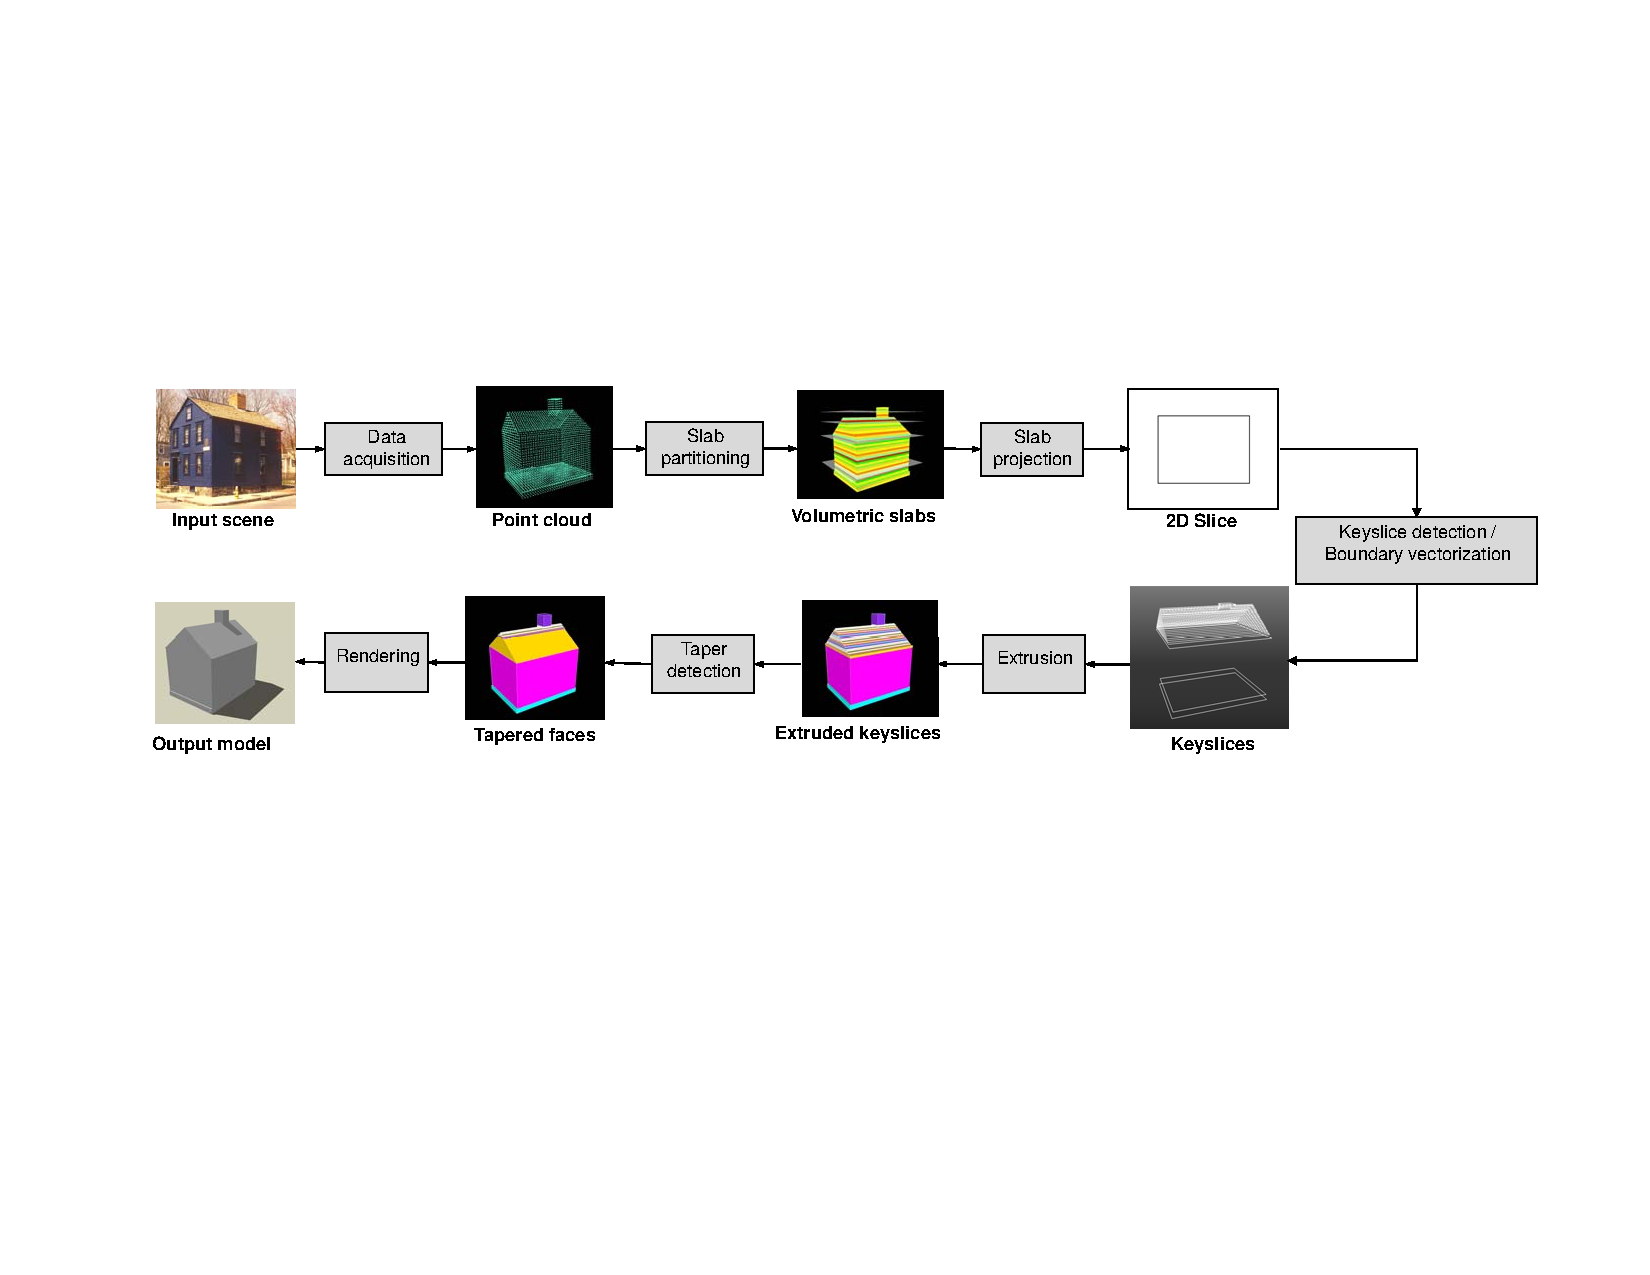
\includegraphics[width=7in]{overview.pdf}
\end{center}
\caption{The basic concept of the proposed method, which only models from bottom-up direction.}
\label{fig:ov}
\end{figure*}

We propose an efficient way to reconstruct 3D models from range data by
partitioning the data into thin cross-sectional volumetric slabs.
For each slab, all range data in that slab is projected onto a 2D
cross-sectional contour slice.
Producing this array of slices permits us to avoid costly computation directly
on 3D data.
A similarity measure is used to cluster the sliced images
together into {\it keyslices}.
This term is analogous to the use of ``keyframes'' in computer animation,
which denote important snapshots in the animation sequence from which
intermediate results can be derived.
In essence, each keyframe is a slice in the spatiotemporal volume of
an animation.
Similarly, each keyslice is a 2D image which contains a {\it transitional}
cross-section of the building, encapsulating major contours in the facade.
The model is then generated by applying basic extrusion and taper
operations from one keyslice to the next.
This produces a lightweight representation consisting of only a few
hundred polygons.

\begin{figure} [htbp]
\begin{center}
\begin{tabular}{c}
\fbox{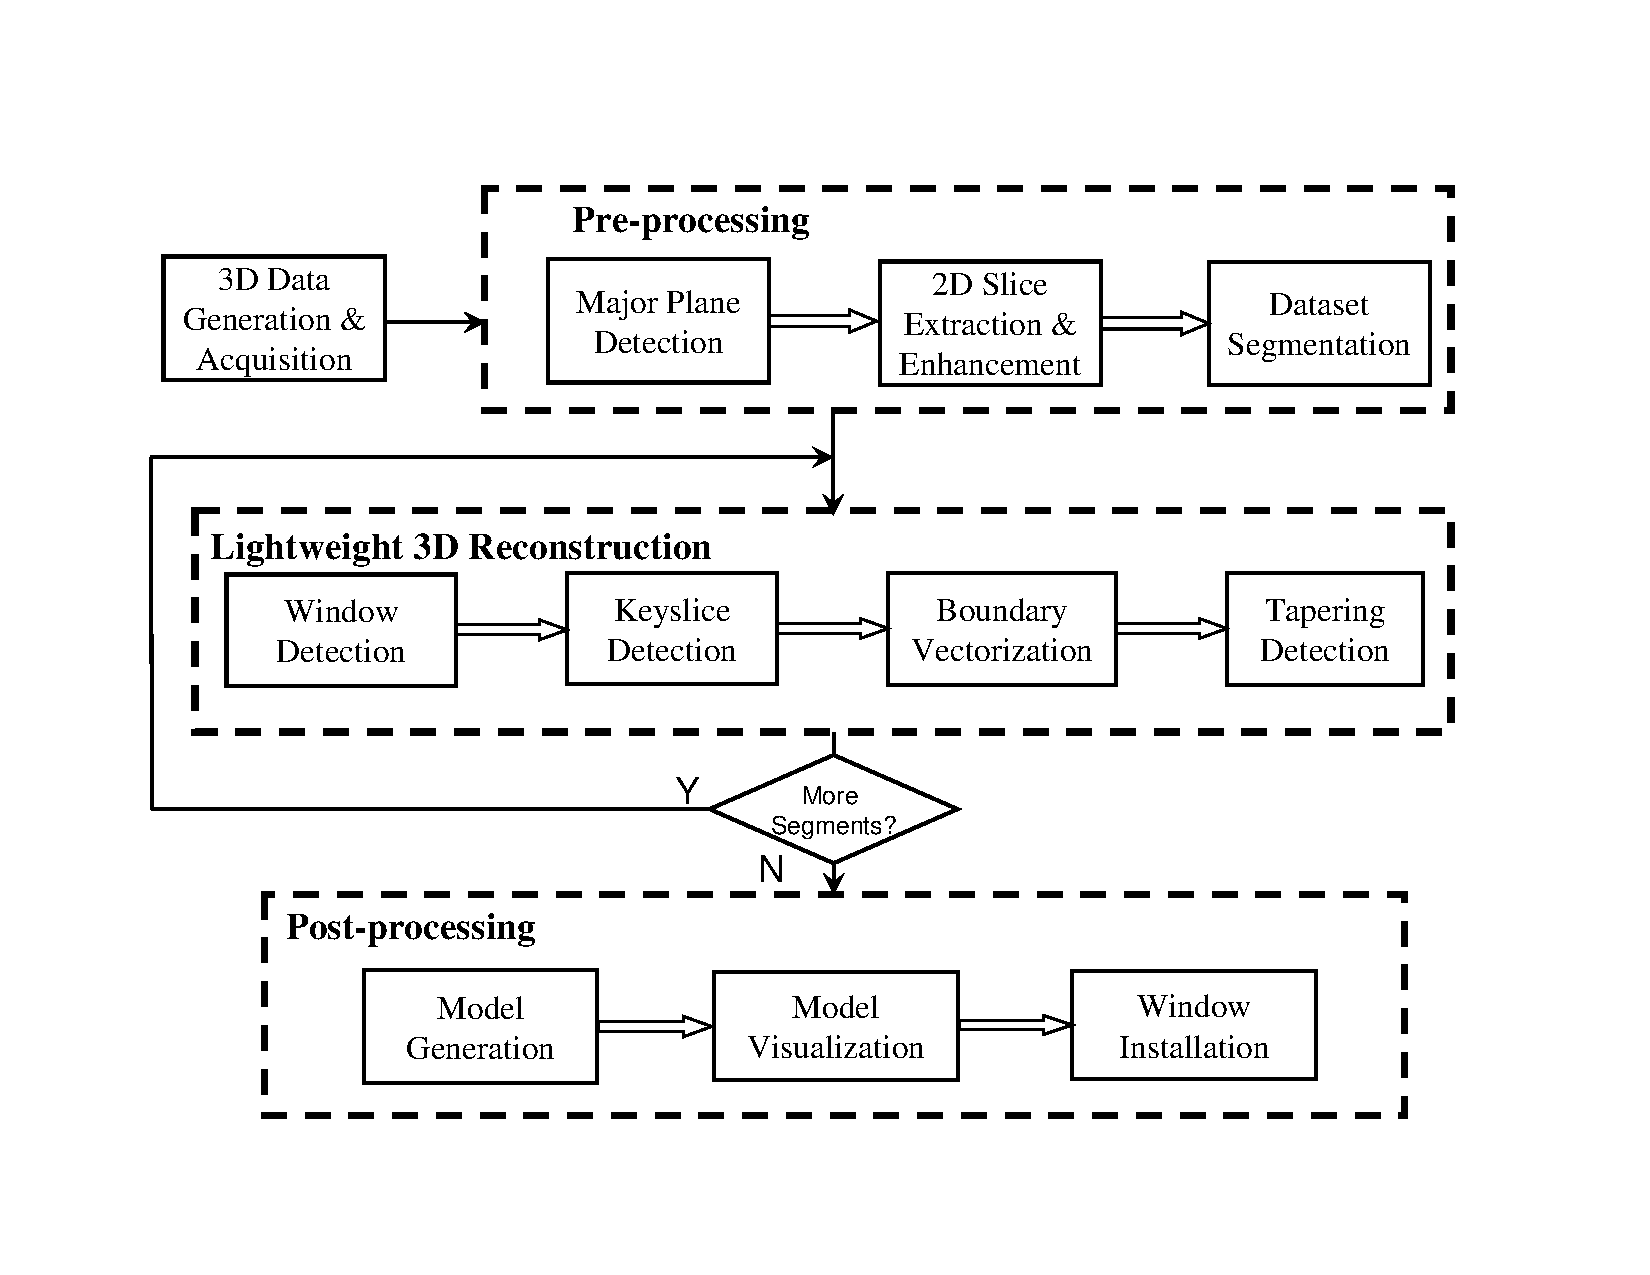
\includegraphics[width=0.45\textwidth]{flow.pdf}}
\end{tabular}
\end{center}
\caption{
The flow diagram of the system, which consists of three stages of processing.
}
\label{fig:flow}
\end{figure}

\Fig{ov} depicts the basic concept of our algorithm. 
We begin with the
acquisition of a dense 3D point cloud $C$ of a building.
$C$ is then partitioned into a nonoverlapping set of volumetric slabs.
Each slab $S$ is associated with one projection plane $P$,
sitting at the base of $S$.
The purpose of partitioning $C$ is to establish a set of cross-sections,
or contour slices.
By examining the changes among these slices, we can identify the prominent
slices, or {\it keyslices}, as well as the necessary extrusion and
taper operations that must apply to them to generate the model.
By casting this 3D modeling task into a series of 2D operations, we
reduce the dimension of the problem to achieve a significant savings in
computational complexity.

The modular flow diagram for our system is shown in \Fig{flow}.
The whole system consists of three stages of computation.
In the first pre-processing stage,
2D slices are extracted from the heavy 3D range data and 
are enhanced by noise removal and the filling of missing data.
The segmentation module is then carried out to divide the complicated
3D dataset into simpler segments.
The second stage is iteratively applied to each segment,
including window detection, keyslice detection, boundary vectorization,
and taper detection.
The final stage is to reconstruct each segment and assemble them into a
whole model.

\subsection{3D Input Data}

The point cloud datasets in our experiments consist of synthetic and real ones. 
The synthetic datasets are generated from 3D building models 
with no noise introduced
and are used for proof of concept. 
These 3D building models which were downloaded from Google SketchUp 3D warehouse 
contain 3D faces and their normals.
The synthetic point cloud can be sampled from these 3D faces as shown in \Figb{syn_data}, 
which consists of approximately 10 million points from the 3D model shown in \Figa{syn_data}.
Because we have the grand truth of reconstructed models, 
that is, the original models, 
the synthetic datasets can also be used to check the correctness and 
measure the errors for reconstructed models. 
On the other hand, the real datasets are acquired from laser scanners.
Due to the nature of buildings (with windows, doors) and blocking, the real 
datasets also contain all kind of noise
and they are only used to validate the proposed approach.


% some key APIs are ..... describe how to download the faces.
\setlength{\tabcolsep}{1.4pt}

\begin{figure}[htbp]
\begin{center}
\begin{tabular}{cc}
        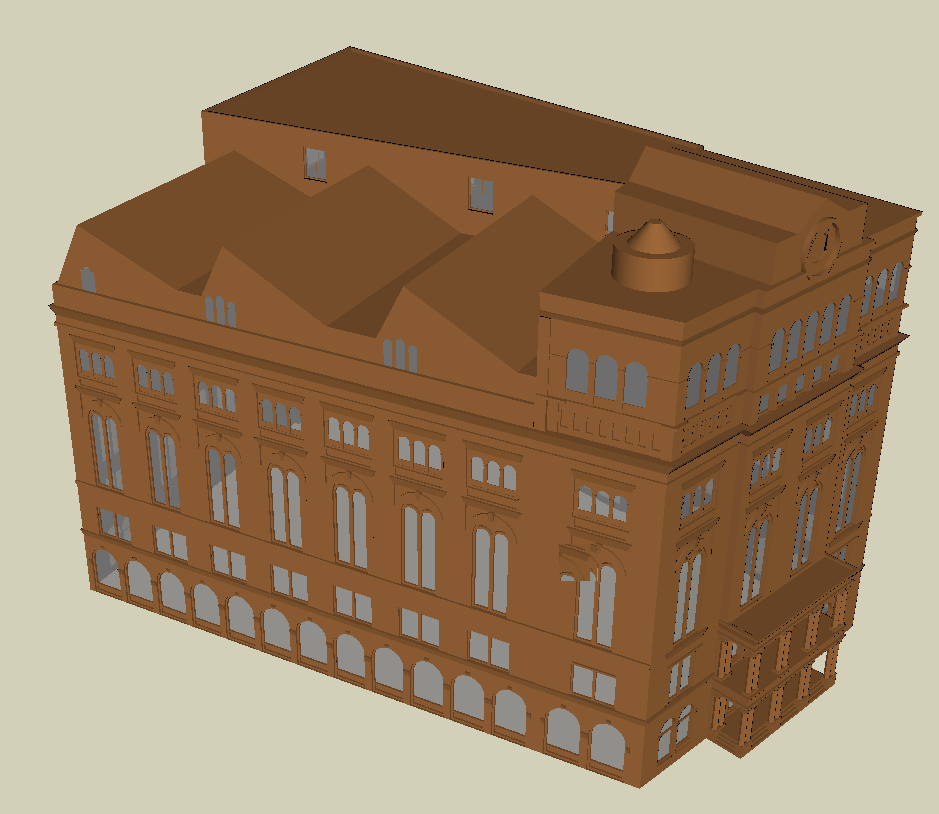
\includegraphics[width=0.2\textwidth]{cu_1.png} &
	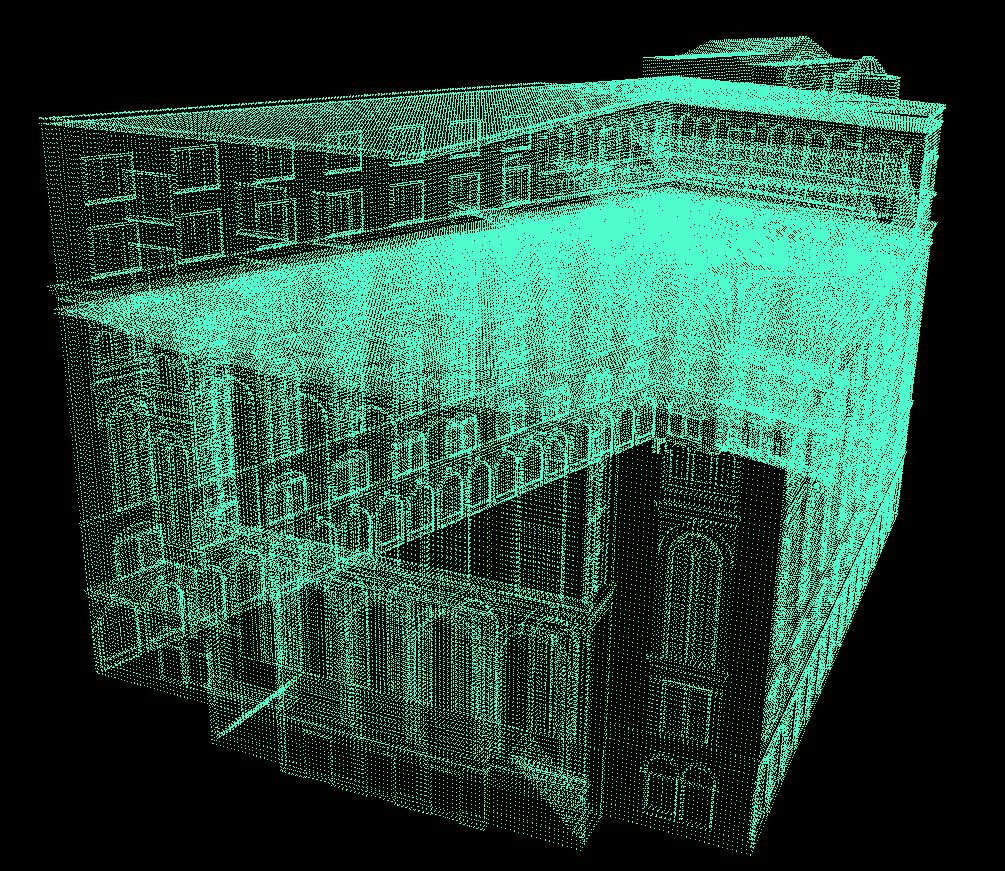
\includegraphics[width=0.2\textwidth]{cu_2.png} \\
	(a) & (b)
\end{tabular}
\end{center}
\caption{
(a) The snapshot of a 3D model.
(b) The snapshot of the synthetic 3D point cloud of for (a).
}
\label{fig:syn_data}
\end{figure}

The real datasets are assembled from range data obtained from 
a Leica Cyrax 2500 laser range scanner \cite{RDP_LRS},
which works by sweeping an eye-safe laser beam across the scene to collect
up to one million 3D depth points per frame.
All scene points that lie within 100 meters can be acquired with an accuracy
of 5mm in depth.
The basic algorithm that we use for registering the voluminous 3D data
acquired from multiple scans of buildings has been introduced in
\cite{RDP_LS}.
That same algorithm is also responsible for extracting the major axes
of the building in order to align it to the axes of the world coordinate
system \cite{RDP_LSYGS}.
This is necessary to properly infer the keyslices.
\Figb{IR_2_DXF} displays a properly aligned, {\it registered} 3D point cloud
consisting of 14 scans totalling 14 million points
collected from \Figa{IR_2_DXF}.

\begin{figure}[htbp]
\begin{center}
\begin{tabular}{cc}
	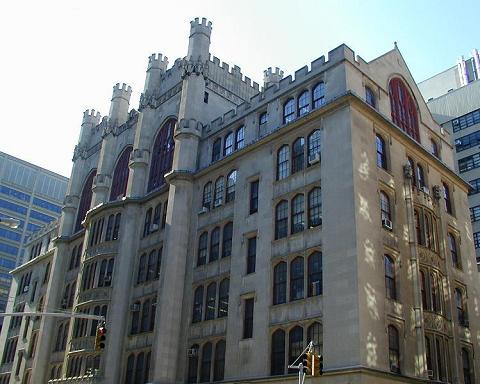
\includegraphics[width=0.22\textwidth]{HunterPhoto.jpg} &
	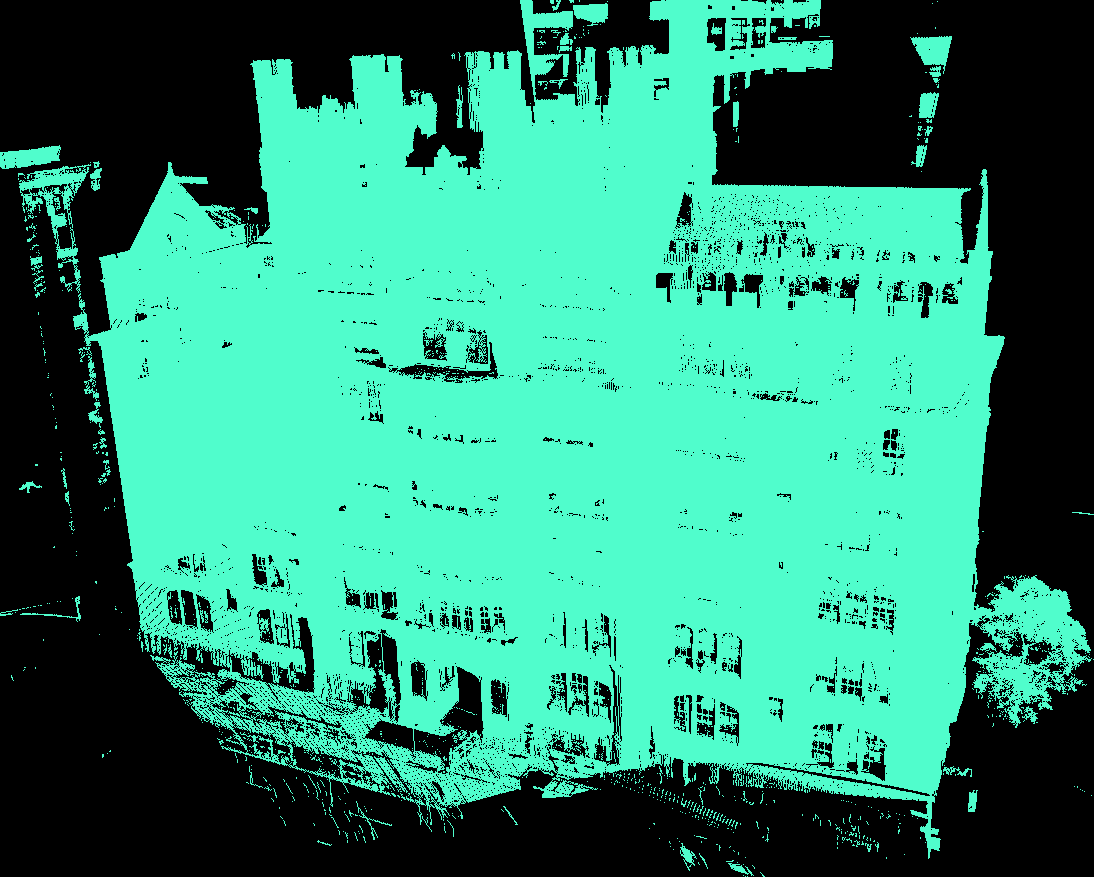
\includegraphics[width=0.22\textwidth]{point_cloud.png} \\
	(a) & (b) \\
\end{tabular}
\end{center}
\caption{
(a) Input scene.
(b) 3D point cloud of scene assembled by registering 14 scans, each having
one million points.
}
\label{fig:IR_2_DXF}
\end{figure}

%%%%%%%%%%%%%%%%%%%%%%%%%%%%%%%%
%%%%%%   PREPROCESSING  %%%%%%%%
%%%%%%%%%%%%%%%%%%%%%%%%%%%%%%%%
\section{Preprocessing the Range Data}
\label{sec:prep}

Due to occlusions and limited vantage points, the point cloud collected by the
laser scanner contains artifacts and holes.
In addition, computing directly on 3D data is time-consuming and
computationally complex.
To tackle these issues, we define inner and outer bounding boxes for the
building to clip away unrelated scene objects.
Then, we convert the 3D modeling problem into a set of 2D problems by
projecting the 3D data into a series of 2D cross-sectional contour images.
Noise removal, hole filling, and vectorization are all done in this
2D space.


\subsection{Major Plane Detection}
\label{sec:major_plane}

The input to our system are unorganized 3D point clouds.
We need to know the major planes in that
these are sweeping direction for extracting 2D slices which
are the starting point for segmentation and window detection.
We used moving least squares (MLS) for deriving a smooth plane from a set
of neighboring data points in space for normal computation.
After the normal is computed for each 3D point, the Hough transform was used
to identify the major plane normals based on voting \cite{MLS01}.
These normals will determine the orientation of the cross-sections that
sweep through the PCD.

\subsection{Extraction of 2D Slices}
\label{sec:image_slicing}

We consider the PCD as a large array of 3D points to be
sliced into parallel volumetric slabs.
All 3D points within each slab are projected onto a projection plane, or slice,
at the base of the slab.
\Fig{slice_slab} shows the 3D point cloud in \Figb{IR_2_DXF} partitioned into
50 slabs.
The projected 3D points in each slab form cross-sectional contour slices.
\Fig{slicing} depicts four such slices, associated with the four displayed
projection planes of \Fig{slice_slab}.

\begin{figure} [htbp]
\begin{center}
\begin{tabular}{c}
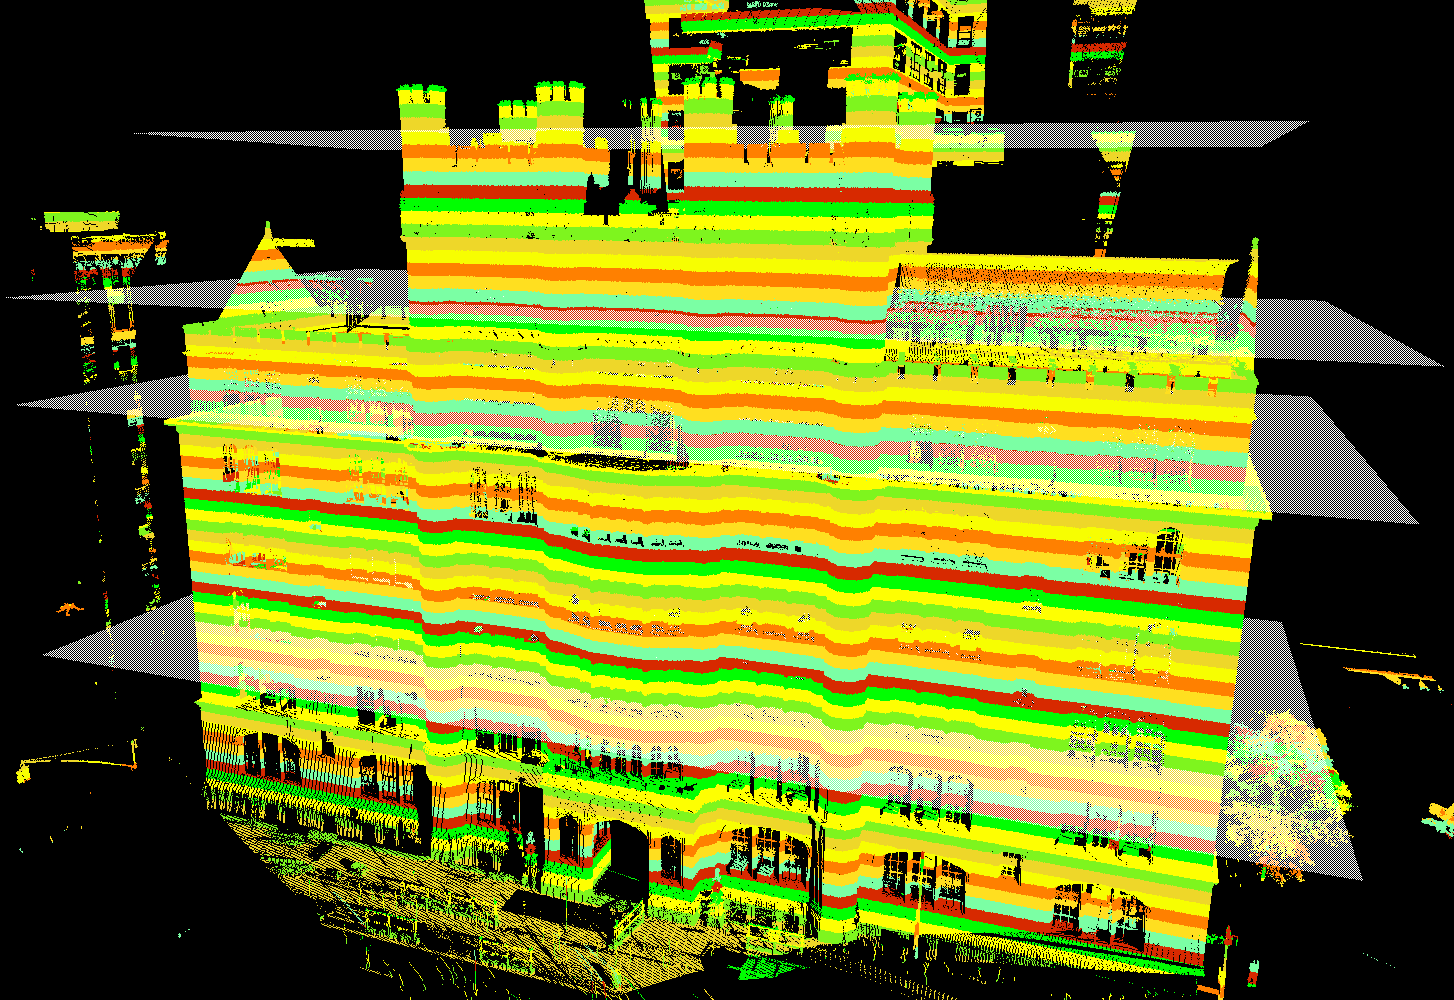
\includegraphics[width=0.35\textwidth]{slab_planar.png} 
\end{tabular}
\end{center}
\caption{The 3D point cloud of \Figb{IR_2_DXF} partitioned into uniform
volumetric slabs.
The 3D points in each slab are projected onto a projection plane to
form cross-sectional slices. Four such planes are shown;
}
\label{fig:slice_slab}
\end{figure}

The height of each slab is $\boldsymbol{\delta}$.
If $\boldsymbol{\delta}$ is held constant, each slice is generated from
equi-spaced slab intervals.
If $\boldsymbol{\delta}$ is allowed to vary, then we may
choose to allow for large values in parts of the structure that are similar,
and low values in regions that contain finer detail.

\begin{figure} [htbp]
\begin{center}
\begin{tabular}{cc}
\fbox{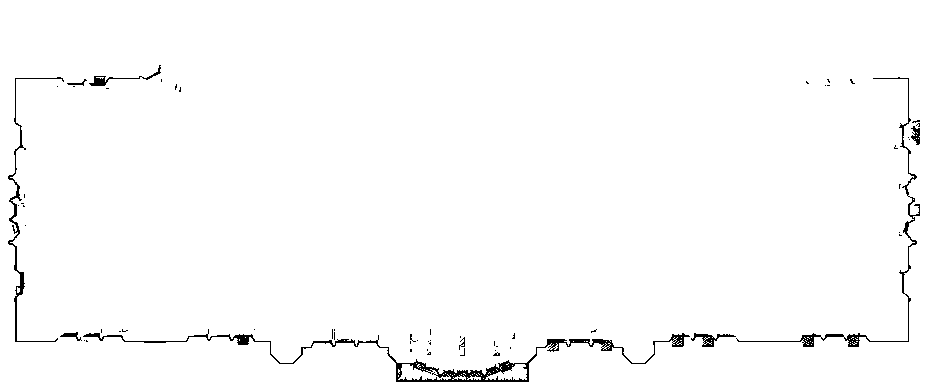
\includegraphics[width=0.22\textwidth]{image_slice_0190.png}} &
\fbox{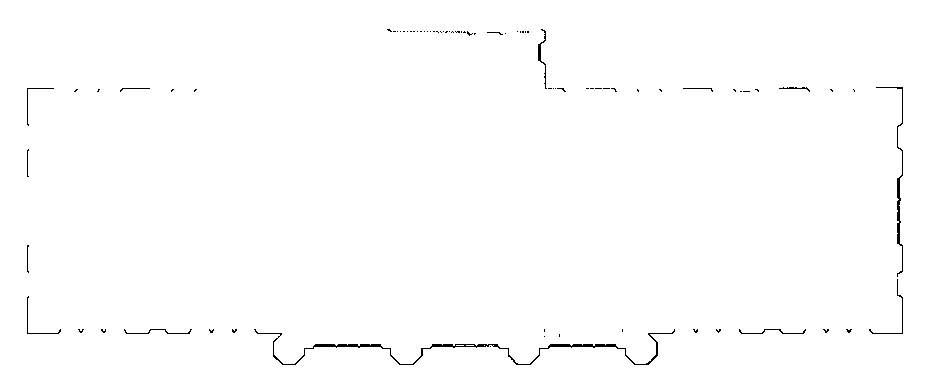
\includegraphics[width=0.22\textwidth]{image_slice_0600.png}} \\
(a) & (b) \\
\fbox{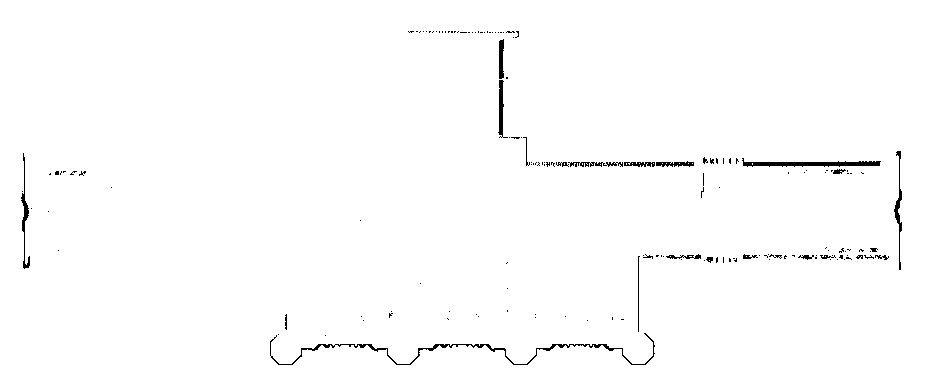
\includegraphics[width=0.22\textwidth]{image_slice_0714.png}} &
\fbox{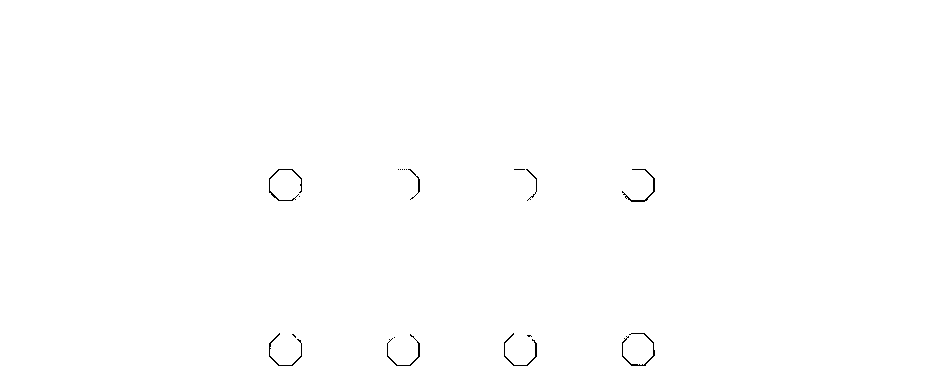
\includegraphics[width=0.22\textwidth]{image_slice_0951.png}} \\
(c) & (d)
\end{tabular}
\end{center}
\caption{The set of slices corresponding to the four projection planes in
\Fig{slice_slab}.}
\label{fig:slicing}
\end{figure}

Without loss of generality, the $y-$axis is used to represent the bottom-up
vertical direction.
Over each slab in height range $[H_{lo}, H_{hi})$,
we project the 3D data $\boldsymbol{P}(x,y,z)$, for $H_{lo} \leq y < H_{hi}$,
onto a 2D image slice.
The projection is normalized in the range $[0,W]$, where $W$ is the image width:
\begin{equation}
[\,x^{2D},\; y^{2D}\,]^T = \omega\cdot[\,x^{3D}_i - X_{MIN},\; z^{3D}_i - Z_{MIN}\,]^T
\label{eq:image_slicing}
\end{equation}
Note that $\omega = W/(X_{MAX} - X_{MIN})$, and that
the [$X_{MIN}$, $X_{MAX}$] and [$Z_{MIN}$, $Z_{MAX}$] pairs define the
3D bounding box, which can be obtained through user input and can be used
to clip away noise data.
\Fig{slicing}(a)-(d) show some examples of the 2D slices, where noise
and incomplete data are observed.
We repeatedly sweep through the volume to extract parallel volumetric slabs
along the directions of the major plane normals computed in \Sec{major_plane}.
\Fig{HT_BPA_Curvature}, for example, depicts slices extracted from the side view.

\subsection{Filling Missing Data}
\label{sec:mdr}

The slices we extract above often have missing data due to
occlusion or other visibility issues.
Fortunately, most urban buildings have symmetry that we can exploit to
fill these gaps.
Symmetry computation on 3D data is expensive \cite{Sym_PSGRF},
so we conduct this computation on the 2D image slices.
Since the 3D data has been already rectified during the registration process
and projected onto 2D slices \cite{Stamos08},
symmetry computation now only needs 2D translation.
Let $P(x,y)$ be a point on the original image $I$ and $P'(x',y')$ be the reflected
point of $P$ with respect to a symmetry line $L$.
The symmetry computation equation for $L$ is as follows:
\begin{equation}
L = \underset{x,y}{\operatorname{arg\,min}}\sum{d_{x,y}(P', I)}
\end{equation}
where $d_{x,y}(P',I)$ is the distance between the self-reflected point
$P'$ and its nearest data point in image $I$.
The reflected point $P'$ of the original point $P$ is computed with
respect to a line along either the $x-$ or $y-$ axis.
Therefore, the symmetry line $L$ is obtained as the line with minimum
summation error over the reflected data points.
\Figa{sym} and \Figb{sym} depict the original input with missing data, and
the output after gap filling using symmetry computation, respectively.

\begin{figure}[htbp]
\begin{center}
\begin{tabular}{cc}
\fbox{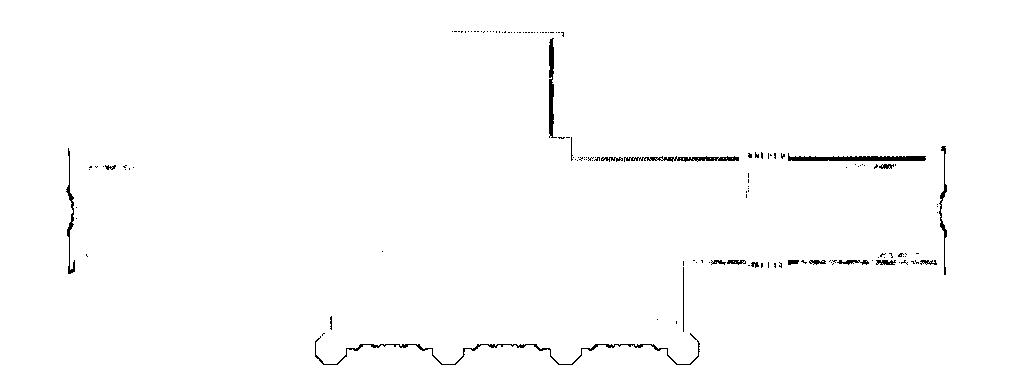
\includegraphics[width=0.22\textwidth]{image_slice_0705_0711.png}} &
\fbox{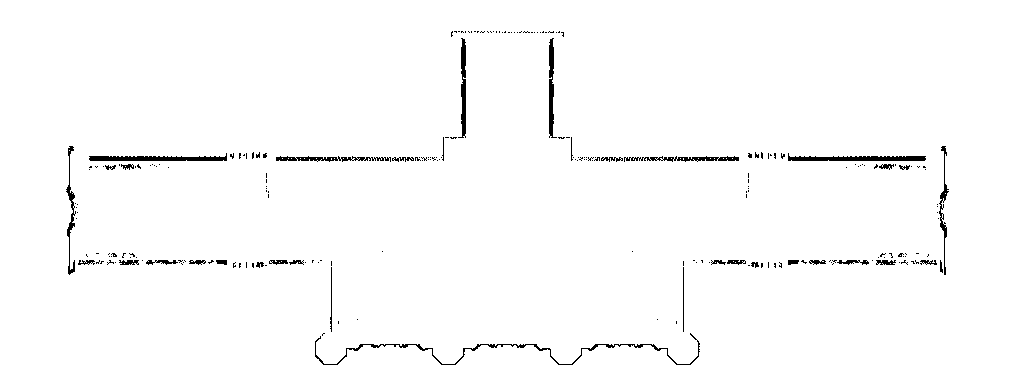
\includegraphics[width=0.22\textwidth]{image_slice_0705_0711_recoverd.png}} \\
(a) & (b)
\end{tabular}
\end{center}
\caption{ Symmetry-based gap filling. (a) Original 2D slice image and
(b) output image after gap filling.}
\label{fig:sym}
\end{figure}

\subsection{Dataset Segmentation}
\label{sec:mseg}

Modeling the PCD of a building as a whole structure simultaneously 
is complicated due to the natural complexity of buildings.
To simplify this problem, we utilize the divide and conquer strategy 
to segment the whole PCD into simpler parts.
We propose an efficient segmentation approach based on the observation 
that different parts of a building are usually separated by walls, ledges,
and other architectural elements.
These {\it ``separators''} provide segmentation clues.
For example, the roof and the body are divided by a ledger as shown in \Figc{MS_Fig1}.
\Figb{MS_Fig1} and \Figd{MS_Fig1} shows different parts of the roof are separated by walls.

\begin{figure}[htbp]
  \centering
  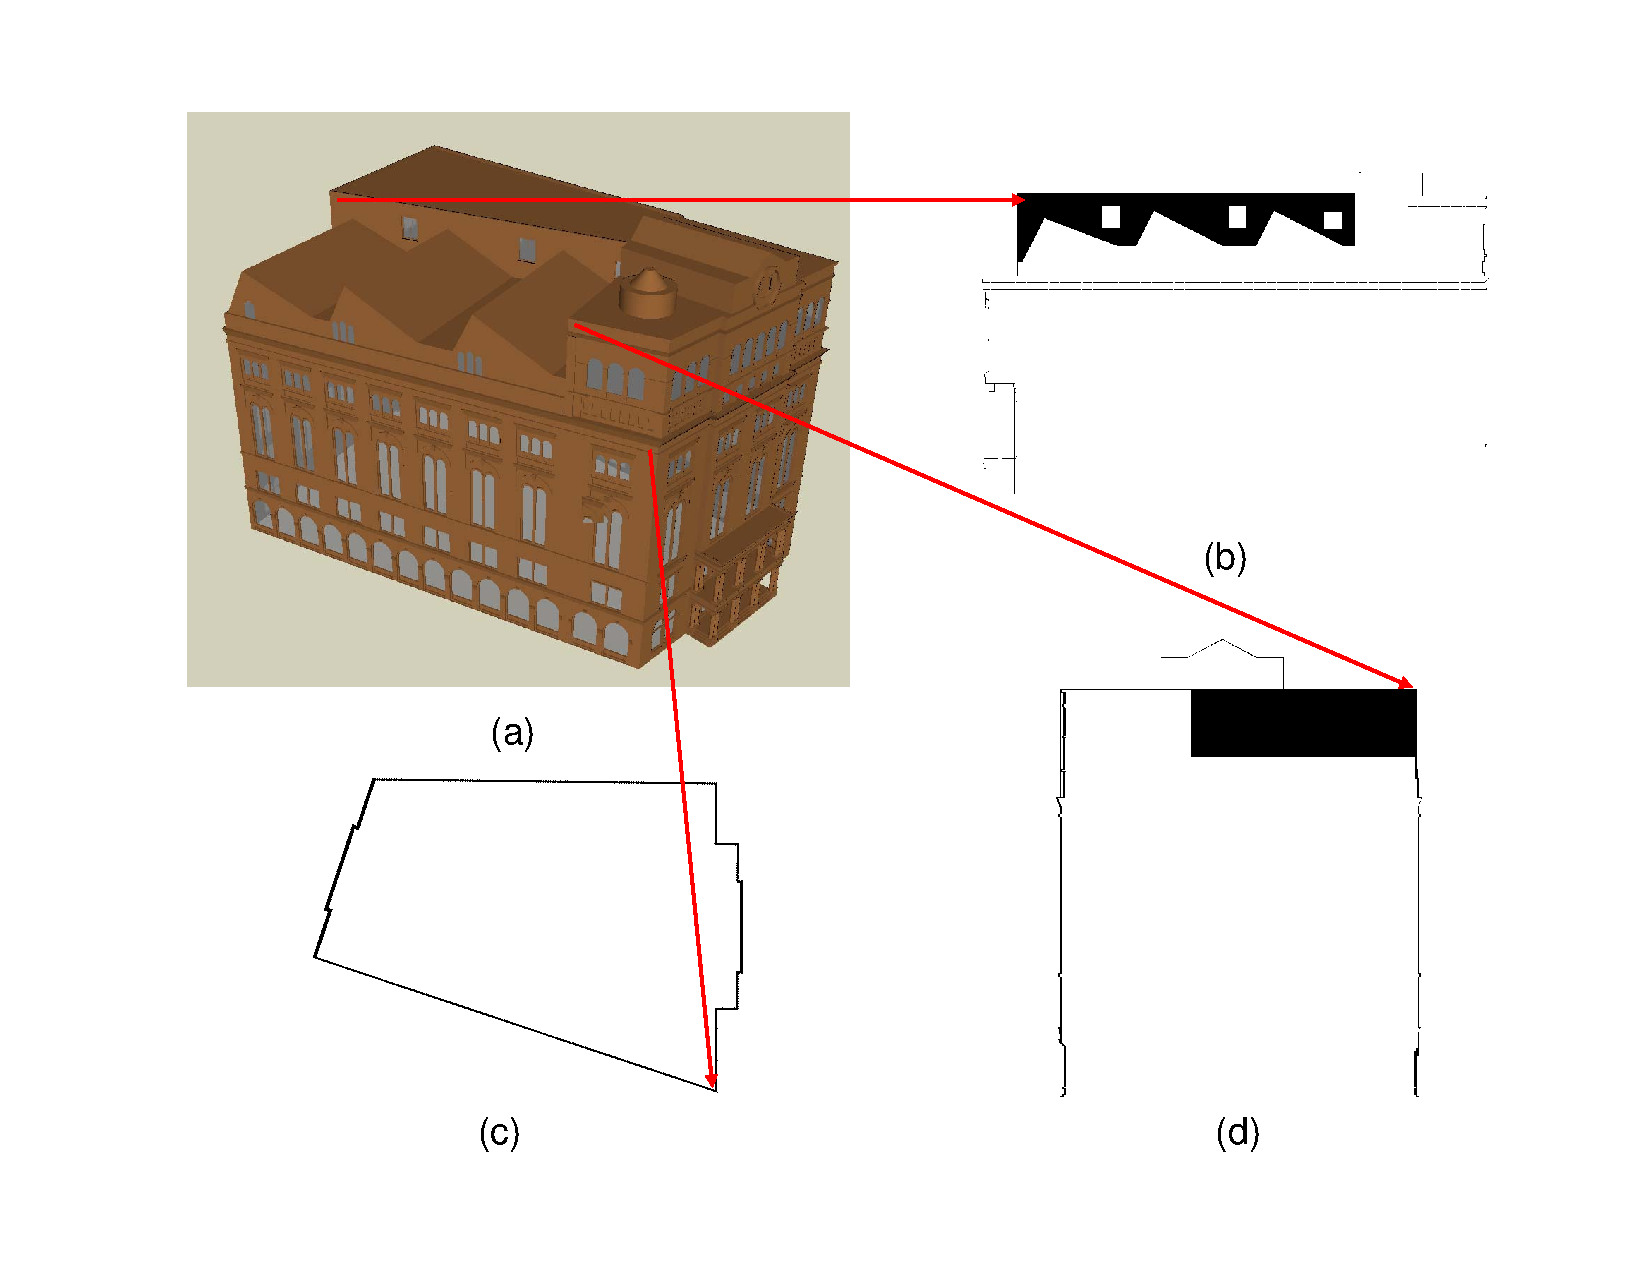
\includegraphics
      [width=0.45\textwidth]
      {model_separate.pdf}
      \caption{The dataset segmentation: 
      (a) the original cooper union model.
      (b) the projected wall image from one face.
      (c) the projected ledger image.
      (d) the projected wall image from another face.}
      \label{fig:MS_Fig1}
\end{figure}

We used a kernel based connected components (CC) method for separators detection.
For each slice image $I_i$, the separator detector
checks each data point $P_i$ using a $5$x$5$ kernel $K$ centered at $P_i$.
Let $S_p$ be a set of points that have been visited by the separator detector.
$S_p$ is initialized to be empty.
The point $P_i$ is checked against $S_p$ to
determine whether it has been visited previously.
If not, $P_i$ is added into $S_p$ and
the data points $N=\{P_j | P_j \neq P_i, P_j \in K\}$
covered by the kernel $K$ are recorded.
If there are enough data points found in the neighbor,
say $|N| > 12$, namely half of the kernel $K$,
$P_i$ is considered as qualified point for the connected component
and is added to $C$.
The same computation is applied to all new recorded data point in $N$,
and qualified points are added into $C$.
When there is no more new data point needs to be checked, the detector stops
and a new connected component, $C$, is detected.

However, for real dataset, separators might be detected in adjacent or
neighboring sliced images as shown in \Figa{segment_merged} - \Figc{segment_merged}.
This is usually caused by imperfect major plane detection
or point cloud data registration introduced in earlier stages.
To cope with this case automatically,
we integrate all the neighboring sliced images
with separators detected into a new image $I$ as shown in \Figd{segment_merged}.
And the same separator detection algorithm is applied on $I$.
The index for this integrated image is set to be the mean
of the indices of those neighboring images.

\begin{figure}[htbp]
\begin{center}
\begin{tabular}{cc}
\fbox{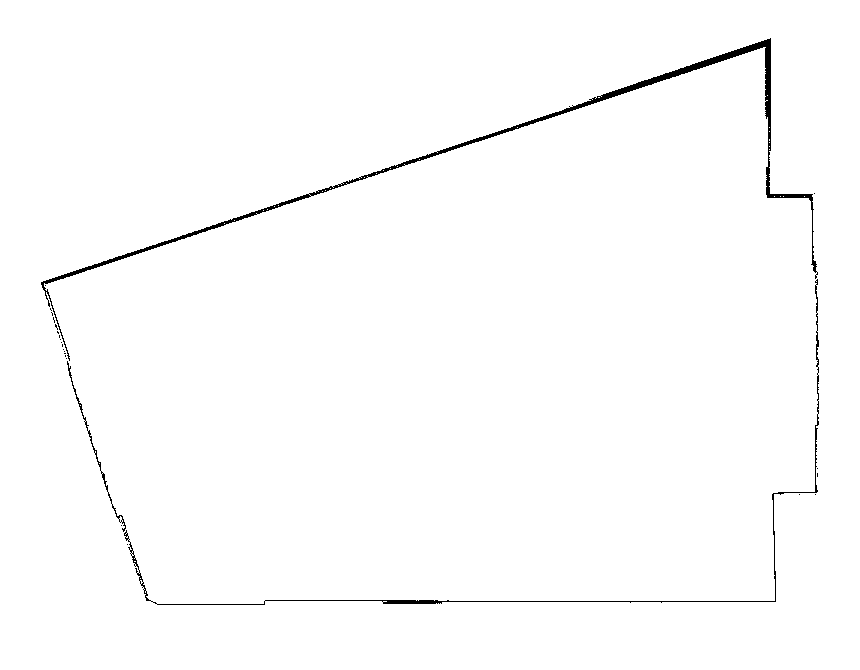
\includegraphics[width=0.2\textwidth]{segment_slice_0091.png}} &
\fbox{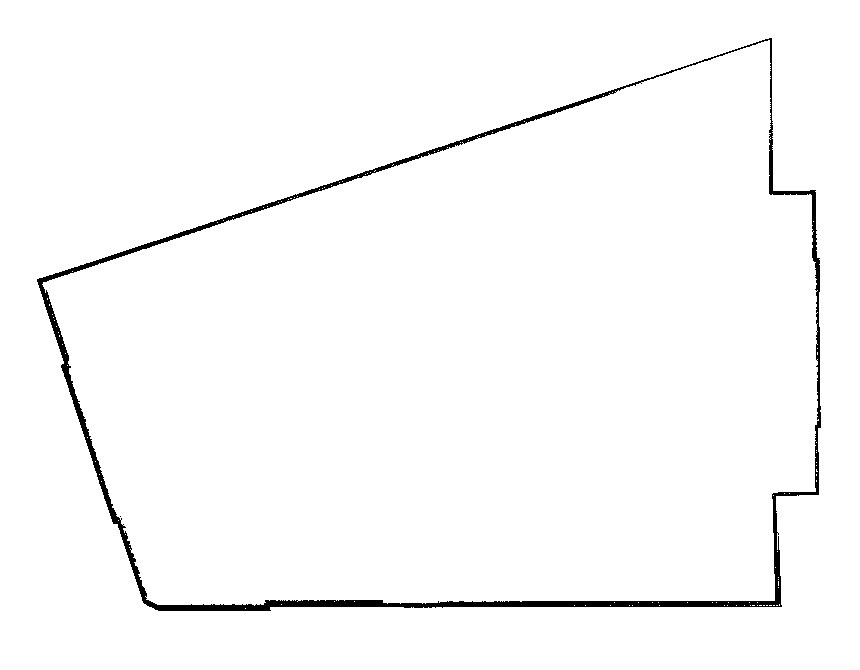
\includegraphics[width=0.2\textwidth]{segment_slice_0092.png}} \\
(a) & (b) \\
\fbox{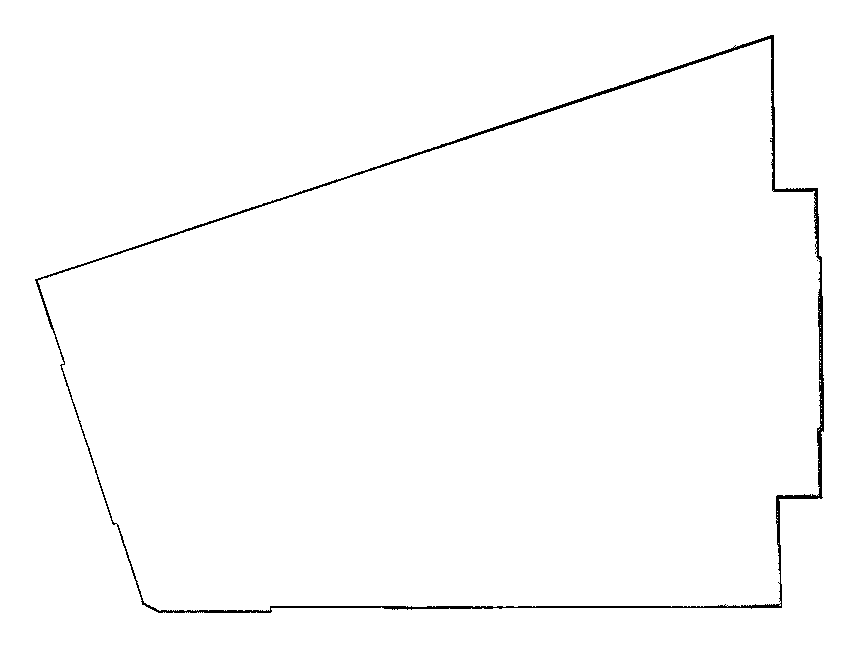
\includegraphics[width=0.2\textwidth]{segment_slice_0093.png}} &
\fbox{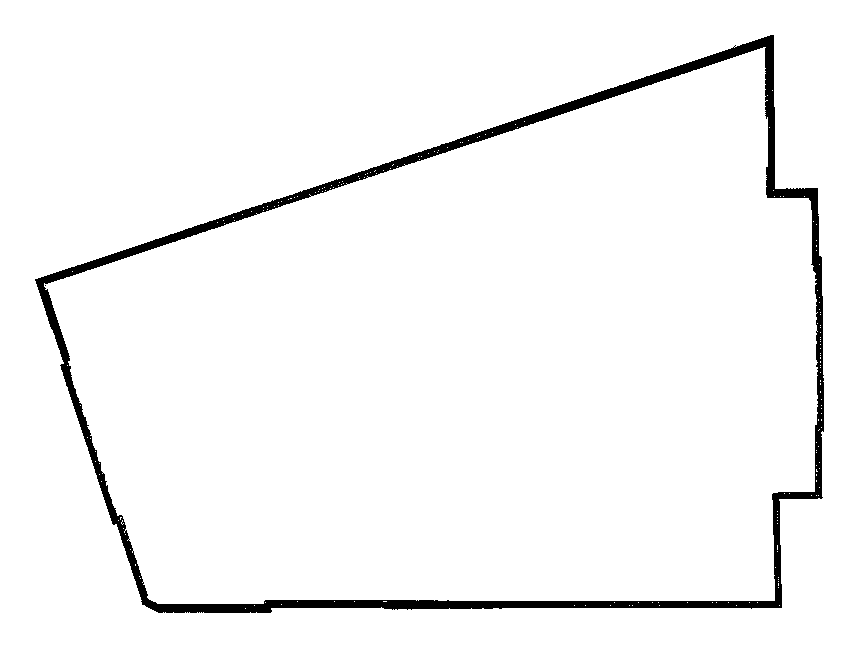
\includegraphics[width=0.2\textwidth]{segment_merged_slice_all.png}} \\
(c) & (d) \\
\end{tabular}
\end{center}
\caption{The adjacent slices with separators detected:
(a) the first slice;
(b) the second consecutive slice;
(c) the third consecutive slice;
(d) the merged slice from (a) to (c).
}
\label{fig:segment_merged}
\end{figure}


%%%%
Once we obtain the separators, we can segment the original dataset based on
the intersections of these separator planes.
First, we need to transform the separators in all directions 
into the common coordinate (with $y$-axis as the bottom-up direction).
Because the separators detected in bottom-up direction
are already in the common coordinate,
no transformation is needed for these separators.
For the example in \Figb{syn_data},
The only detected separator (the ledger) as shown in \Figc{MS_Fig1}
divides the whole dataset into top (roof structure) and
bottom (body structure).

%% other directions
For other directions, each separator is transformed into 
a line segment in the bottom-up projected image.
The roof and body projected images are shown in 
\Figa{DS_Fig1} and \Figb{DS_Fig1} respectively.
To compute the boundary for each segment,
the intersection points 
for each line segment with other line segments are computed.
After intersection points are computed for all line segments, 
the segmentation image $I_s$ can be obtained.
\Figc{DS_Fig1} and \Figd{DS_Fig1} illustrate the computed segmentation images
for both body and roof sections.
Different regions are marked in different colors 
and are assigned a unique region id. 

\begin{figure} [htbp]
\begin{center}
\begin{tabular}{cccc}
\fbox{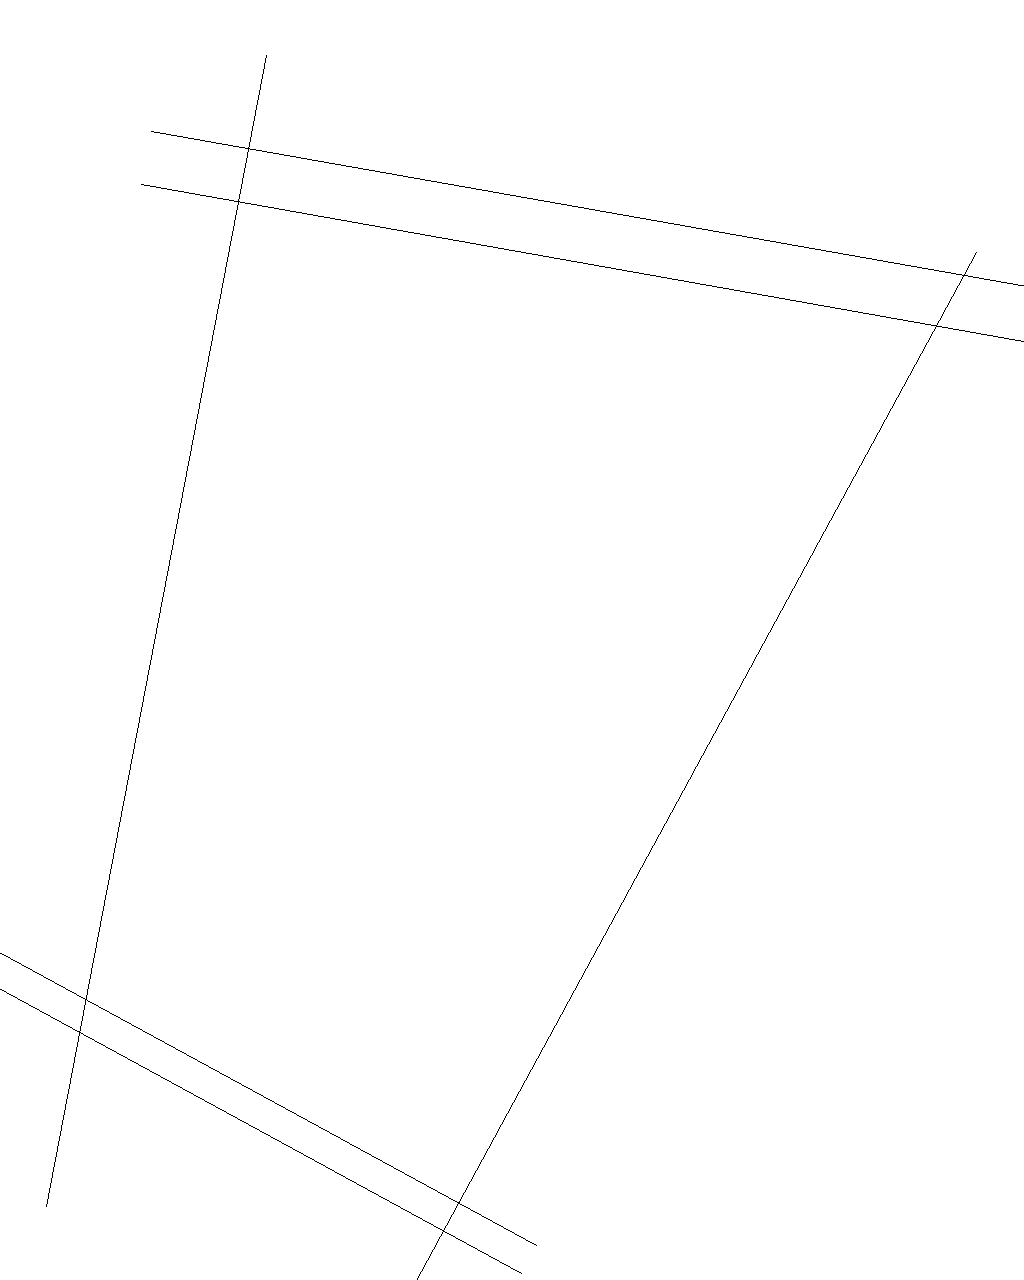
\includegraphics[width=0.1\textwidth]{segment_body_result.png}} &
\fbox{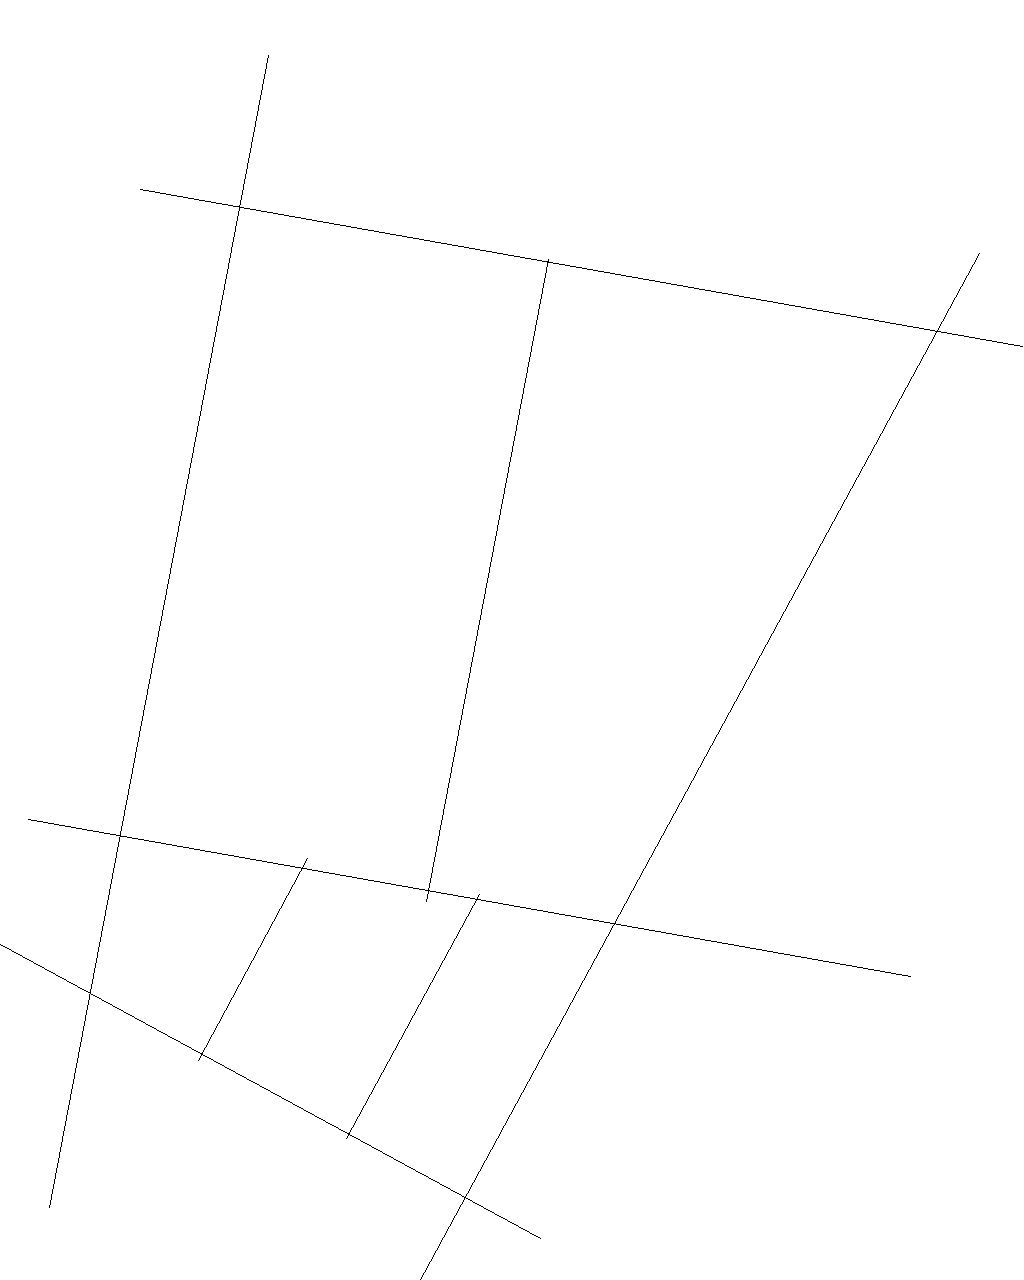
\includegraphics[width=0.1\textwidth]{segment_roof_result.png}} &
\fbox{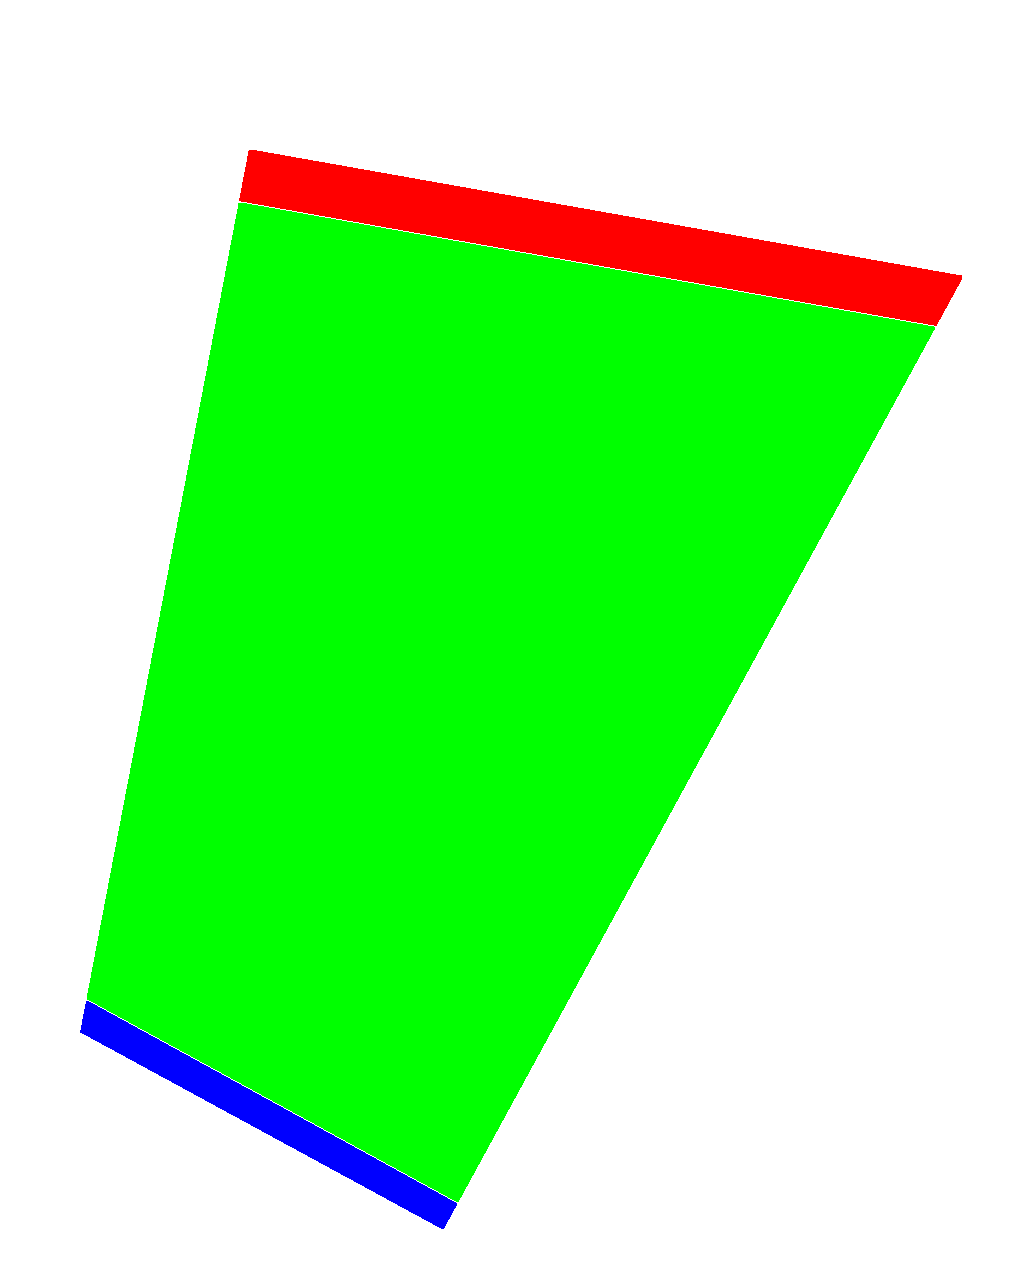
\includegraphics[width=0.1\textwidth]{segment_body_regions.png}} &
\fbox{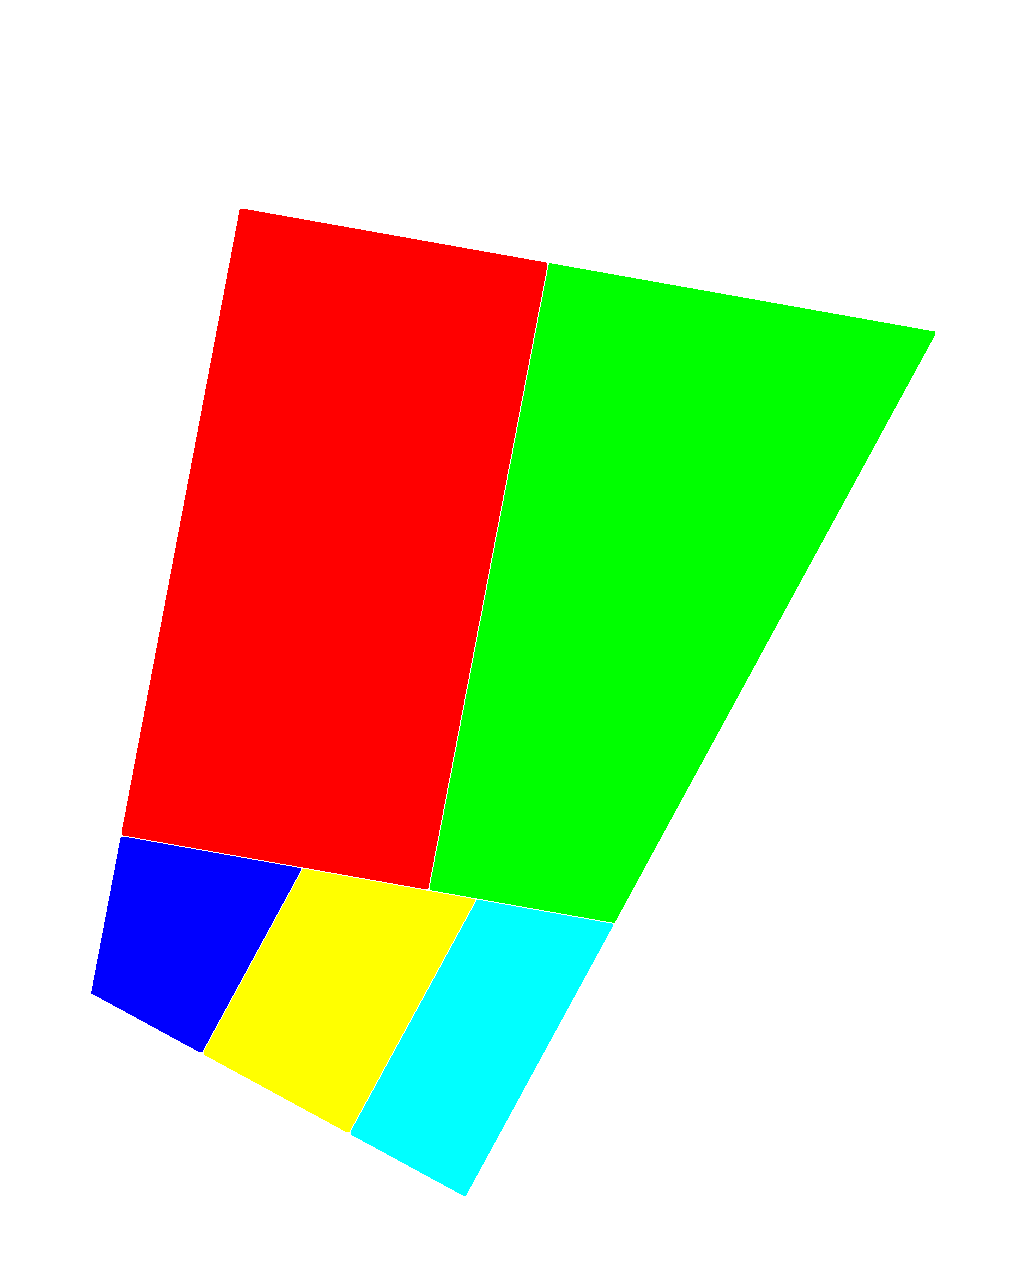
\includegraphics[width=0.1\textwidth]{segment_roof_regions.png}} \\
(a) & (b) & (c) & (d) 
\end{tabular}
\end{center}
\caption{ Segmentation region computation:
      (a) the transformed image with line segment of the separators for body,
      (b) the transformed image with line segment of the separators for roof,
      (c) the processed segment image regions for body,
      (d) the processed segment image regions for roof. }
\label{fig:DS_Fig1}
\end{figure}

For each 3D data point ${\bf P}(x, y, z)$, 
we first compute its group in bottom-up direction
by comparing ${\bf P}$'s $y$ value (bottom-up direction) and 
those heights from range indices.
Once the group is computed, with the segmentation image $I_s$, 
we can further compute the region id for ${\bf P}$ by
obtaining its 2D projection point $P(x, y)$ in the image $I_s$. 
The region id for $P$ can be obtained from the look-up table $T$.
\Fig{results} column (c) show the 3D segmentation results,
where different segments are labeled with different colors.

%%%%%%%%%%%%%%%%%%%%%%%%%%%%%%%%
%%%%%%   3D Reconstruction  %%%%
%%%%%%%%%%%%%%%%%%%%%%%%%%%%%%%%
\section{Lightweight 3D Reconstruction}
\label{sec:reconst}
Our 3D modeling algorithm is based on \emph{a priori} knowledge that
urban buildings can be created through a series of extrusion and taper
operations on the salient cross-sections contained in the keyslices.
The main step for successful modeling is identifying these salient cross
sections upon which the extrusion and taper operations apply.

\subsection{Window Detection}
\label{sec:wdd}
Windows and doors are important features for buildings to be modeled.
Without knowing the locations of the windows, extra keyslices may be computed 
hence leading to excessive extrusion operations on windows.
Image-based windows and doors detection has been widely conducted in 
\cite{WDD_LN,WDD_TKKJ}.
Essentially, the 2D window regions are extracted by exploiting the properties
of building structures, such as shape and symmetry. 
The estimation of the depth for the extracted 2D windows is computed 
by using matches for the linear features within the extracted
window in two or more ground views.
However, the estimation is not reliable due to perspective projection.
Some window detection methods on 3D data have also been proposed in
\cite{WDD_SV,WDD_BBH}.
A constrained surface fitting and a genetic algorithm 
is proposed to fit parametric models of doors on point cloud in \cite{WDD_FF}.
This method assumes that the data have been segmented 
and requires relatively high density data around the window area.
Pu and Vosselman use a triangulation-based method 
to detect the boundaries of sparse regions within a building facade 
and then fit rectangles to the resulting region to compute windows \cite{WDD_PV}.
Our window computation is based on the work presented in \cite{WDD_PV}.

Following this, we can generate mask images based on the boundaries of the
detected windows to discard those points for keyslice computation.
The mask images can be generated by fusing all the window information. 
\Fig{WD_Fig3} shows couple of mask image examples 
for different height range of the cross-sectional slices.
Note that the regions circled in red illustrate the major differences
between mask images, which are caused by the different cross-sectional
structures viewed from different locations.

\begin{figure}[htbp]
\begin{center}
\begin{tabular}{cc}
\fbox{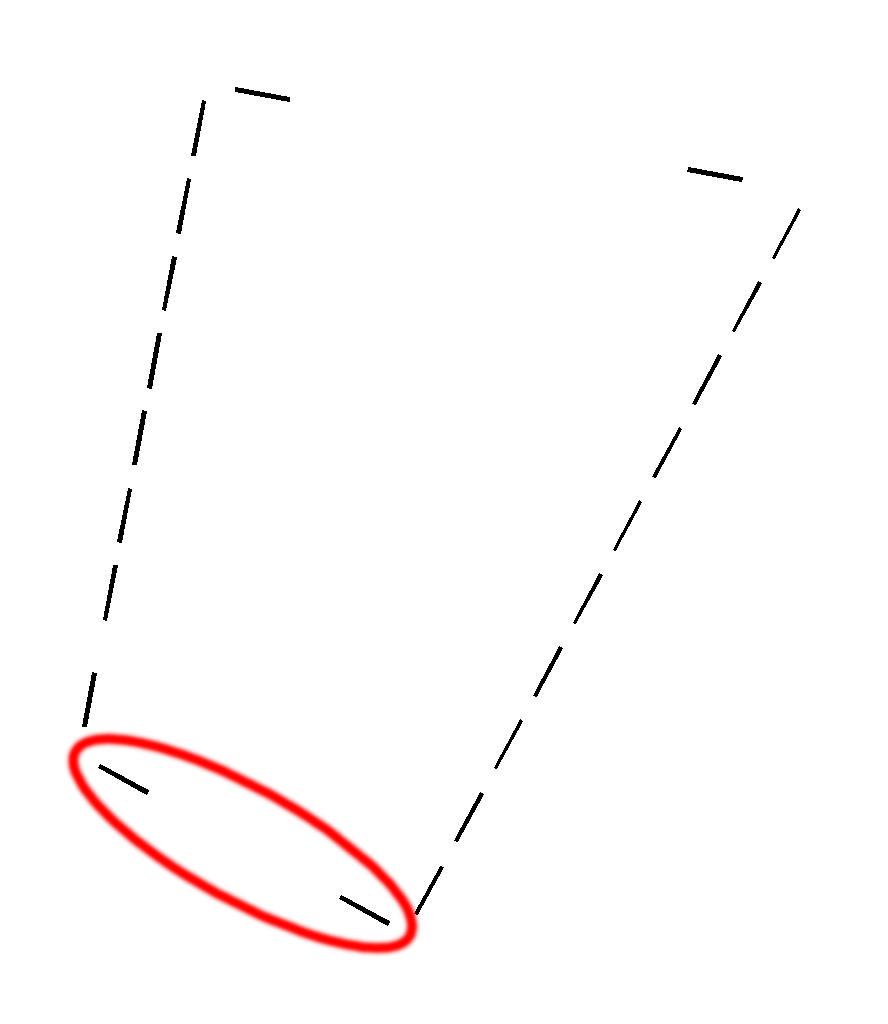
\includegraphics[width=0.20\textwidth]{window_mask_1.jpg}} &
\fbox{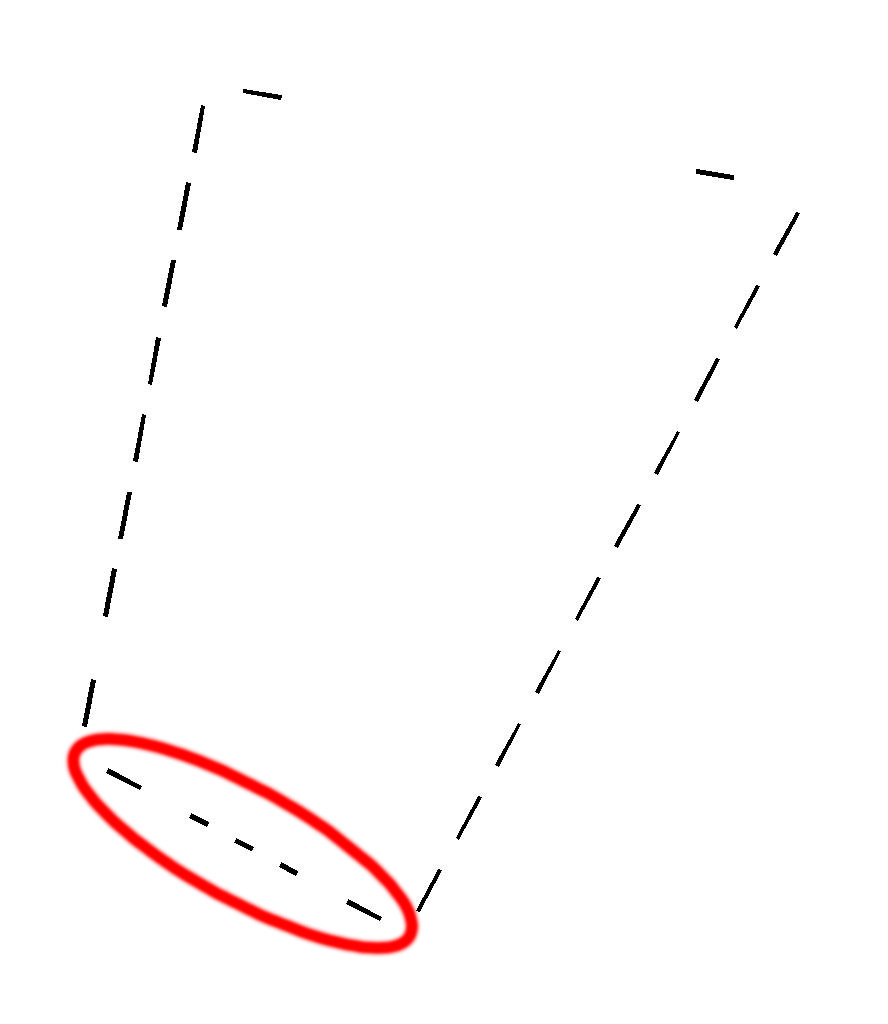
\includegraphics[width=0.20\textwidth]{window_mask_2.jpg}} \\
(a) & (b)
\end{tabular}
\end{center}
\caption{The window mask images: 
         (a) The mask image corresponding to height range of bottom windows.
	 (b) The mask image corresponding to height range of upper windows.}
\label{fig:WD_Fig3}
\end{figure}

\subsection{Keyslice Detection}
\label{sec:ksd}

The 2D image slices of an extruded region are similar to each other.
To detect the keyslices that delimit extruded regions one only needs
to compute the similarity between adjacent slices.
We select the Hausdorff distance as the similarity measure.
Let $P_r(x_r, y_r)$ and $P_i(x_i, y_i)$ be a data point in 
a reference image and a new observed image $I$, respectively.
The Hausdorff distance of image $I$ to reference image $I_r$ is defined as:
\begin{equation}
d_H(I, I_r) = \sum_{i=0}^Nd_{min}(P_i, I_r)
\label{eq:hd}
\end{equation}
where $d_{min}(P_i, I_r)$ is the minimum distance from $P_i$ in image $I$
to the reference image $I_r$.
Alternatively, we can also define the Hausdorff distance, $d_H(I_r, I)$,
from $I_r$ to a new observed image $I$, using \Eq{hd}.
These two distances are usually not equal to each other.
As a rule of thumb, one can choose
$d_{HD} = \text{MAX}\{d_H(I, I_r), d_H(I_r, I)\}$ as the Hausdorff distance.
To compute the keyslices, a threshold $\tau_{d}$ is used for the
Hausdorff distance $d_{HD}$.
If $d_{HD} < \tau_{d}$, the two images $I$ and $I_r$ are considered
similar to each other.
Otherwise, a keyslice image is found and $I_r$ is updated with $I$,
the new keyslice image.

The accuracy of the keyslices detected by using the Hausdorff distance
is closely tied to threshold $\tau_d$.
Small $\tau_d$ leads to more accurate models and will require more time and
space to compute and store the result.
When the threshold $\tau_d$ is relatively large, potential keyslices which
contain salient structure may be missed.
Therefore, there is a trade-off between model accuracy and time-space
efficiency.
To address this problem, the curvature information is computed as a
complementary criteria for keyslice detection.

This idea is based on the observation that the keyslices are generally
located at large curvature changes along 2D slices extracted in the orthogonal
direction (e.g., side view), as shown in \Figa{HT_BPA_Curvature}.
Therefore, instead of computing the difference between two images directly,
we compute the curvature of orthogonal 2D slices, map the positions of
curvature extrema back to cross-sections in the original set of volumetric
slabs, and mark these cross-sections as keyslices.

\begin{figure}[htbp]
\centerline{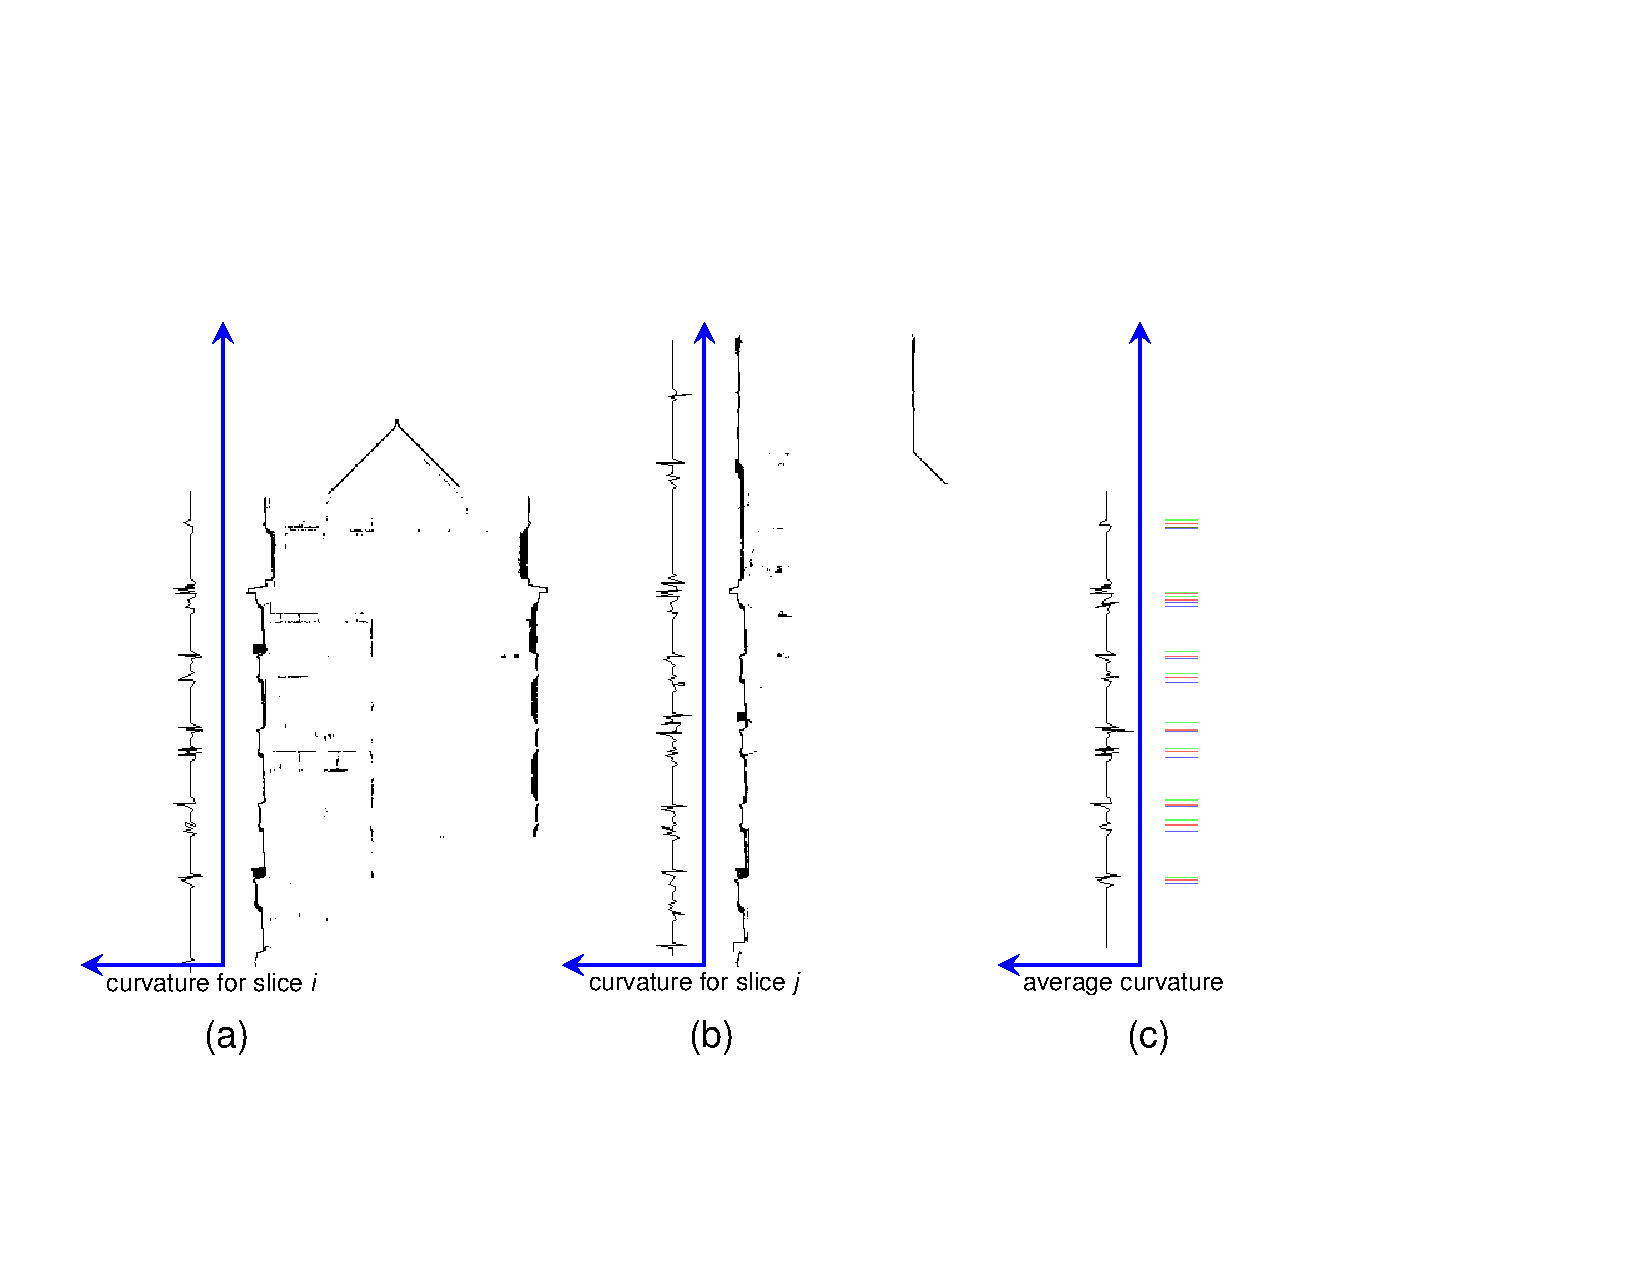
\includegraphics[width=.5\textwidth]{curvature_comp.pdf}}
\caption{Curvature-based key slice detection.
(a,b) Two 2D sliced images from the orthogonal direction (side view).
A plot of the curvature of each slice is displayed alongside.
(c) A plot of the average curvatures detected over all of the sliced
images along the orthogonal direction.
Thresholding the curvature yields the location of keyslices, displayed
alongside the plot.
Red lines along the average curvature plot indicate local maxima.
Blue and green lines, respectively, indicate zero-crossings in the
average curvature.
This delineates the keyslice positions.
}
\label{fig:HT_BPA_Curvature}
\end{figure}

To compute the curvature, we first apply the slice extraction algorithm
described in \Sec{image_slicing} to obtain a series of 2D cross-sectional
images in the orthogonal direction.
We then apply the ball-pivoting algorithm described in \Sec{BPA} to
vectorize the boundary for each sliced image.
We locate those curvatures that appear in most of the sliced images as the
places where keyslices are found, as shown in \Figb{HT_BPA_Curvature}.
Note that the red lines indicate the location of the center of the curvature,
and the blue and green lines indicate the entering and exiting of the
curvature structures, respectively.
The combination of Hausdorff distance measurement and curvature inference
ensures that the salient structures of a building will be preserved.

\subsection{Boundary Vectorization}
\label{sec:BPA}

After the keyslices are detected, 
$N_K$ keyslices will be identified from a total of $N_A$ image slices.
Depending on the threshold $\tau_d$, 
$N_K$ is usually about one to two orders of magnitude smaller than $N_A$, 
e.g., $N_K/N_A$ is 0.06 when $\tau_d$ = 4.0 
for the example in \Figb{IR_2_DXF}.
To generate the 3D model, 
these keyslice images need to be vectorized to
represent the contours of the building facade.
The difficulty of the problem lies in outliers and holes of non-perfect images.
We proposed a general framework based on an adaptive 2D ball-pivot algorithm (BPA) 
 to efficiently suppress the noisy, 
fill holes and 
generate contours for those images.

\subsubsection{Ball Pivot Algorithm}

Raster image vectorization has been an active research topic
and some classical methods are widely used 
in digital image processing for years, 
such as those described in \cite{DP_RP}.
However, these approaches only consider 
the cases where perfect raster image data is provided.
For non-perfect data, these proposed methods were failed in various cases.
The problem considered here is to compute contours
for non-perfect binary images which may contain holes
along the boundary as well as noise or outliers
inside the boundary. Here, {\it boundary} refers to the
out-most region of any raster image and
{\it contour} refers to a vectorized boundary.


\begin{figure}[htbp]
\begin{center}
\begin{tabular}{cc}
\fbox{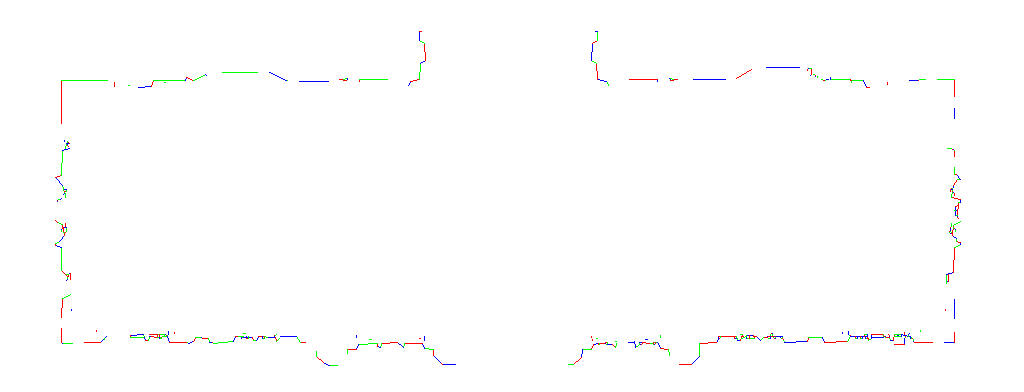
\includegraphics[width=0.22\textwidth]{failed_case_ply.png}} &
\fbox{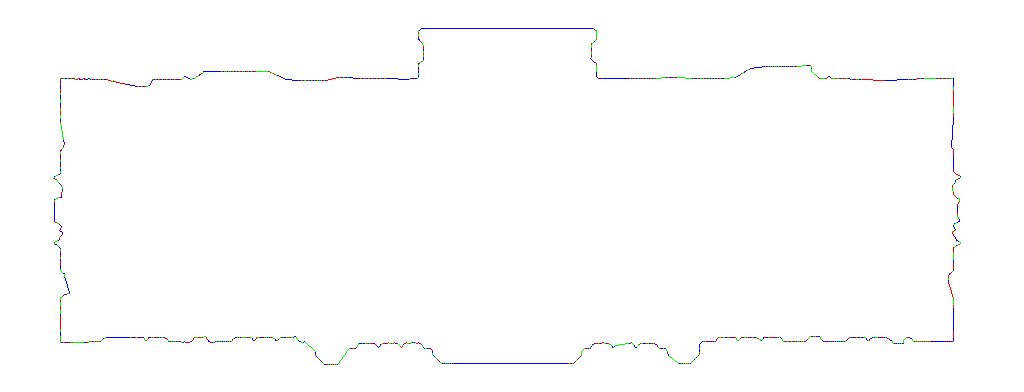
\includegraphics[width=0.22\textwidth]{failed_case_bpa.png}} \\
(a) & (b) 
\end{tabular}
\end{center}
\caption{
(a) The vectorization result based on DP algorithm and
(b) The vectorization result from proposed BPA algorithm.}
\label{fig:failed_case}
\end{figure}


The Douglas-Peucker (DP) algorithm \cite{DP_DP} is widely used
to compute boundary vectorization for binary images.
Although the complexity of this approach is $O(nlogn)$ after 
the improvement of implementation described in \cite{DP_HS94},
this method cannot fill the holes of the noisy data or 
handle the case where spurious interior points are presented.
For example, \Figb{failed_case} shows the contour 
generated from DP algorithm from a binary cross-sectional image. 
The problem is that there are
a lot of holes along the contour and the noise inside of the
boundary are modeled inappropriately.

\begin{figure}[hbtp]
\begin{center}
\begin{tabular}{cc}
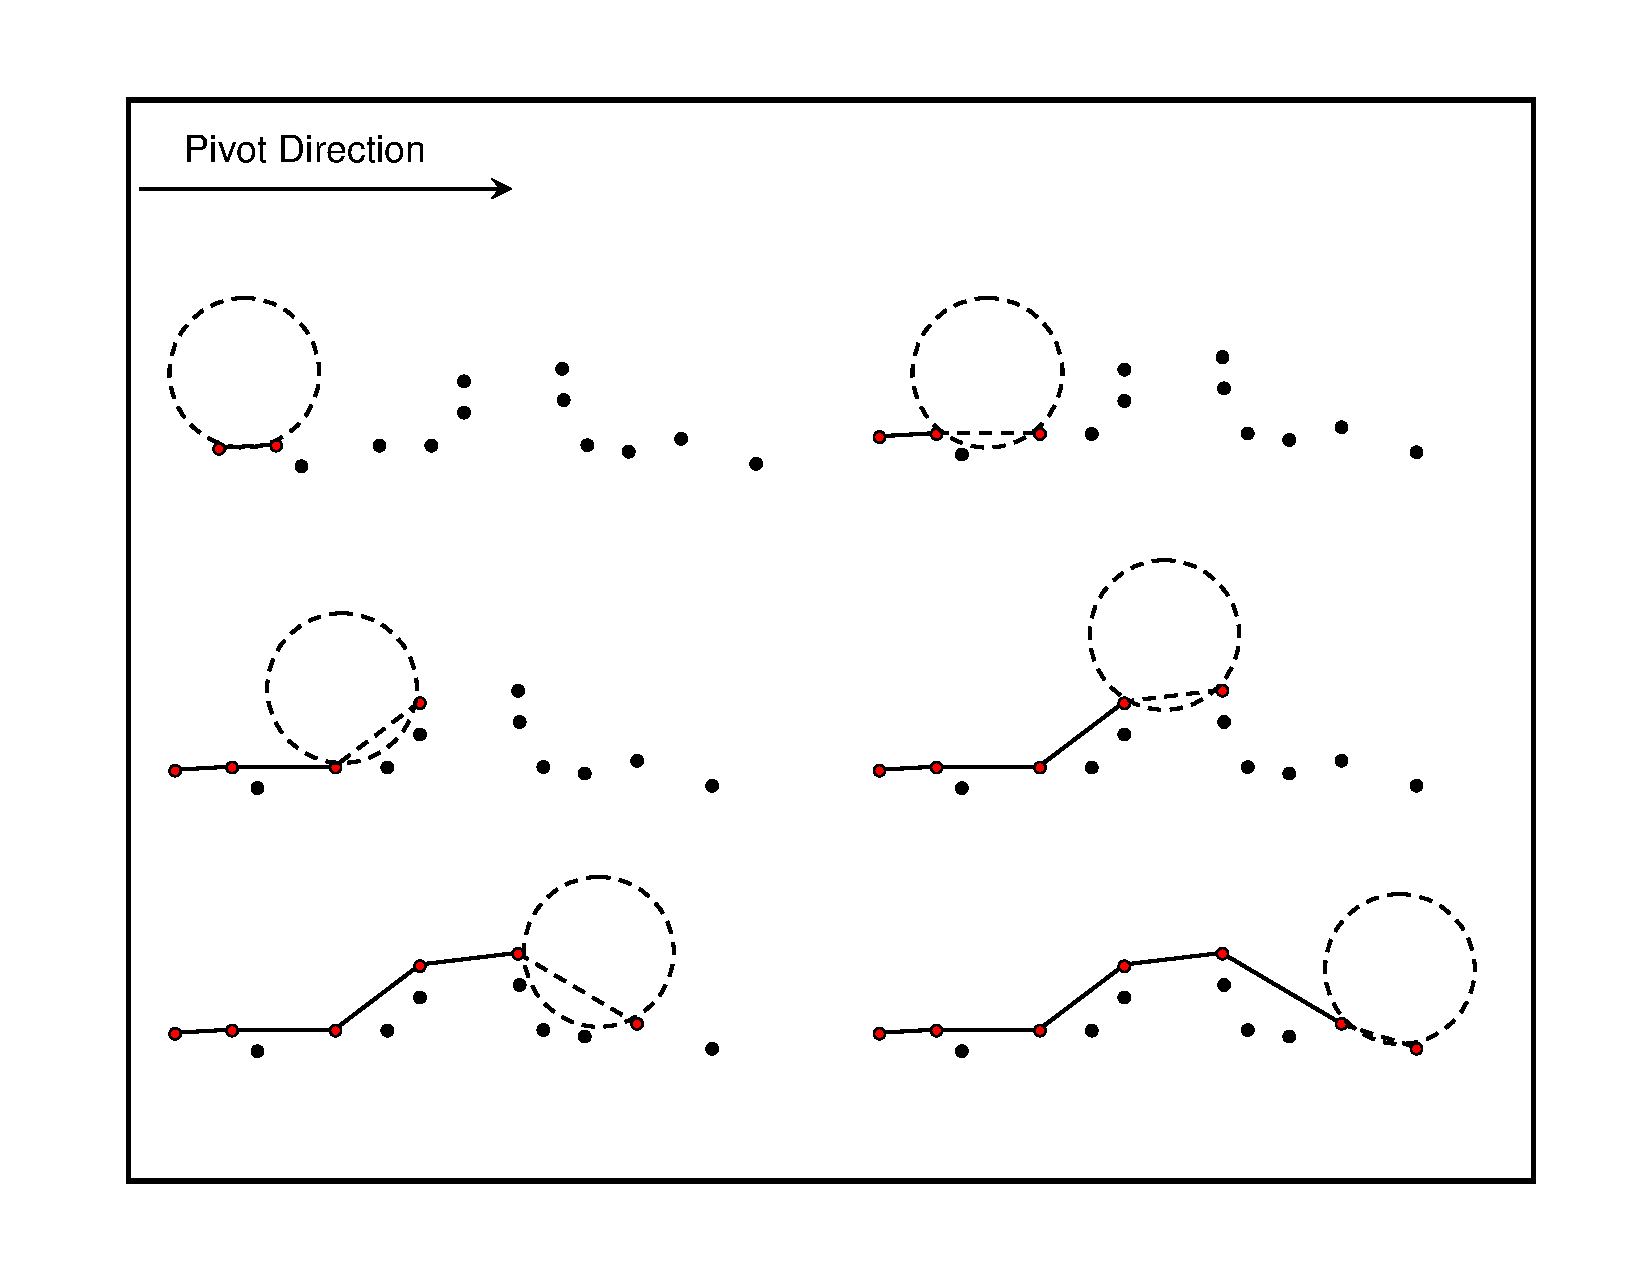
\includegraphics[width=0.24\textwidth]{BPA_init.pdf} &
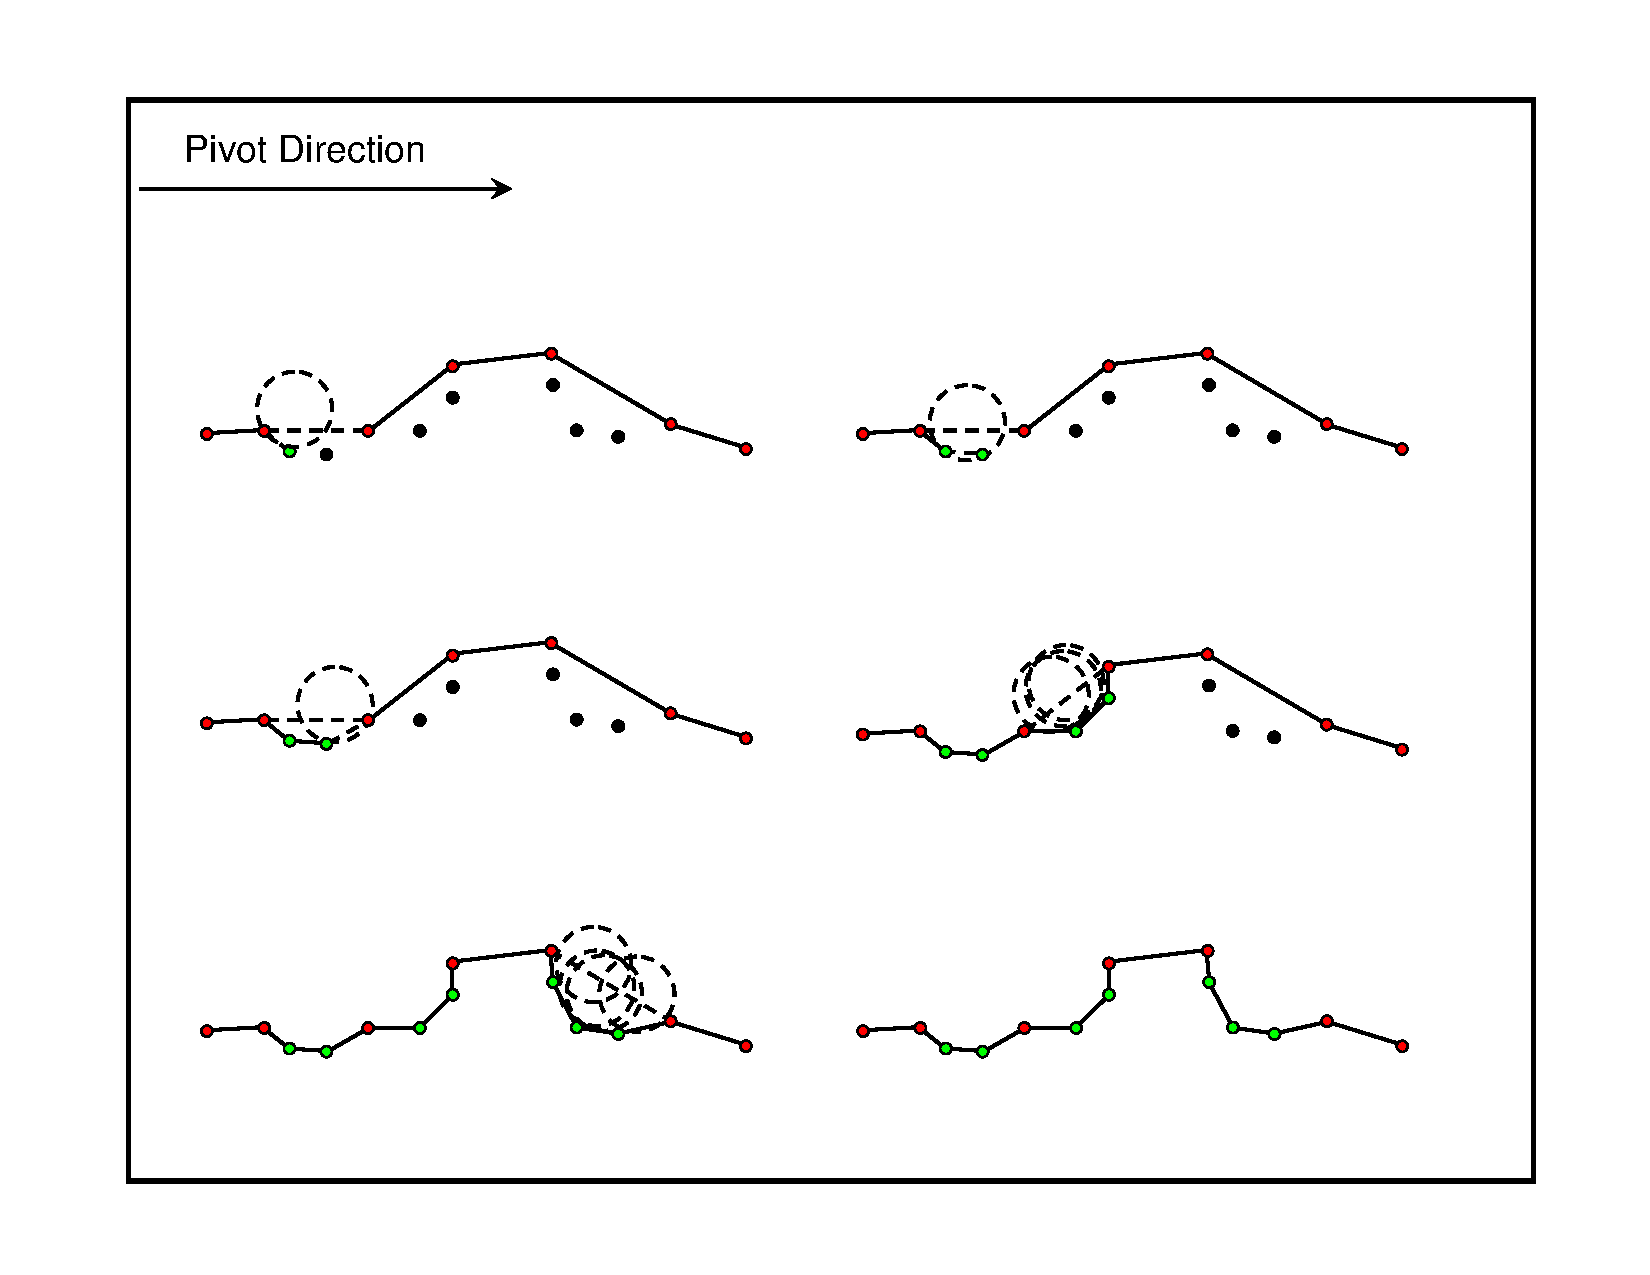
\includegraphics[width=0.24\textwidth]{BPA_refine.pdf} \\
(a) & (b)
\end{tabular}
\end{center}
\caption{Adaptive ball pivoting algorithm:
(a) Initial pivoting with a ball of radius 2$r$;
(b) Refinement with a ball of radius $r$.}
\label{fig:BPA}
\end{figure}


The original Ball Pivot Algorithm (BPA) was proposed to efficiently 
generate 3D mesh representation on 3D point cloud data.
The 2D BPA algorithm works well and efficiently on 
computing contours with appropriate parameters.
The key parameter for BPA to work successfully is 
the size of the ball for pivoting.
We have proposed an adaptive BPA to address this problem.
\Figb{failed_case} shows
the contour computed by the proposed method which fills holes between gaps
and suppresses noise inside the boundary.

The idea of the BPA is straight-forward:
pivot a ball on a starting point in the image
until it touches another data point as depicted in \Figa{BPA}.
Add the new touched
data point into an ordered list as the vertices of the contour polygon and
set it as the new pivoting point.
Keep doing this pivoting process until all data points are touched.

\subsubsection{Boundary Vectorization}

The basic idea behind the proposed framework 
for contour computation is as follows:
apply BPA on a selected starting point until
either the ball pivots back to the starting point 
which indicates a closed boundary is detected,
or the ball reaches a gap which means this contour is a non-closed
contour and one of the end points is reached.
Because the ball can start pivoting along either clock-wise direction 
or counter clock-wise direction,
another pivoting process at start pivoting from 
the alternative direction is conducted.
When both directions have been explored, 
a contour computation is done.
After this, a {\it refinement} process is carried out 
for each line segments using the same BPA algorithm.
For this refinement, the starting point is now 
the first end point of a line
and the stopping case is that the ball reaches the other point 
or it reaches a gap as depicted in \Figb{BPA}.

\subsubsection{Contour Simplification}
\label{sec:BPA_HT}
%%% Adaptive BPA + HT %%%%

Although the proposed framework is an efficient and straightforward 
approach to vectorize the contours of noisy images,
it produces many short line segments which can be merged.
In particular, when the underlying boundary is a straight line structure,
the BPA produces excessive un-necessary short lines due to its way 
of generating the contour.
An example is shown in the upper part of the contour in \Figa{HT_BPA_figure}
where each colored segment represents a contour edge.
One way to reduce the number of vertices of the polygon is to apply
the approximation polygon method in \cite{DP_AV}. 
The drawback of this method is that the topological structures, 
such as straight lines, would be lost.
Therefore, we combined the proposed 2D BPA and the Hough transform
to replace short line segments with long lines and eliminate noisy
or outlier vertices around the boundary.

\begin{figure}[htbp]
\begin{center}
\begin{tabular}{cc}
\fbox{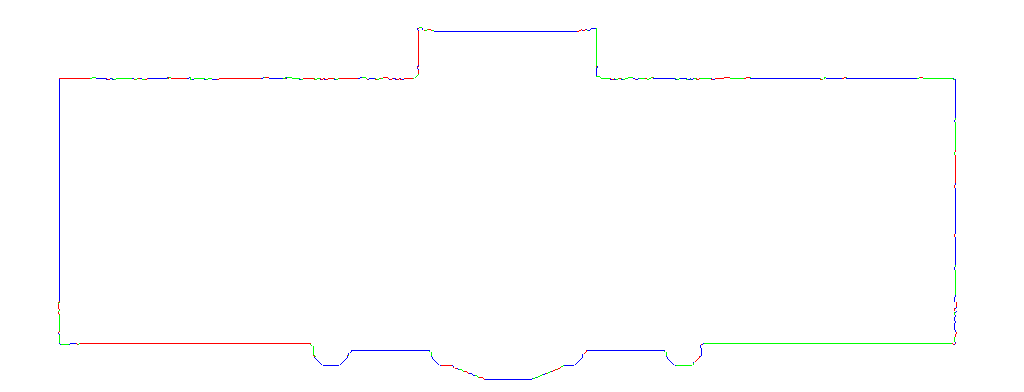
\includegraphics[width=0.22\textwidth]
{bbb_image_slice_1024_392_0533_refine_with_rad_1_and_merged.png}} &
\fbox{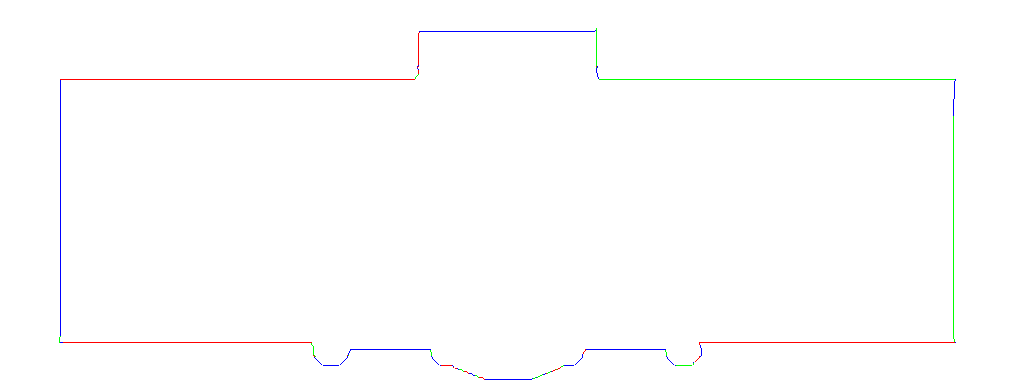
\includegraphics[width=0.22\textwidth]
{bbb_image_slice_1024_392_0533_combine_HT_BPA_rad_32.png}} \\
(a) & (b)
\end{tabular}
\end{center}
\caption{Boundary vectorization of noisy binary image.
(a) the contour computed by ABPA method only.
(b) the contour obtained by simplification with Hough transform.}
\label{fig:HT_BPA_figure}
\end{figure}

After the integration of BPA contour with the Hough transform lines,
the beautified contour is shown in \Figb{HT_BPA_figure}.
Notice that the top part of the contour, 
which consists of short line segments, 
was replaced with two long line segments.
As one can see, this process reduces the noise, 
simplifies the contour, 
and produces clean results 
for contours with straight line structures.

\subsection{Extrusion and Taper Detection}
\label{sec:tsd}

After the keyslices are detected and vectorized, the contours of
${\bf N_K} = \{I_i | i = 0, ..., K \}$ keyslices are used to represent
the building based on the extrusion operation.
That is, the space between each pair of keyslices, say $I_{i}$ and $I_{j}$,
can be interpolated by the lower keyslice, e.g., $I_{i}$ in this case.
This is valid because of the similarity between the intermediate slices
and the keyslice $I_{i}$.
By modeling a building using this series of keyslices ${\bf N_K}$, 
we significantly reduce the number of polygons for urban buildings. 

In addition to the extrusion operation, we can further improve
the model and reduce the model size based on the observation
that part of the keyslice images may belong to the same tapered structure.
\Figa{DXF_top} shows the roof structure of the reconstructed model 
from a keyslice image extrusion operation with
almost half of the keyslices dedicated to the tapered structure.
After inferring the tapered structure, 
\Figb{DXF_top} shows the improvement of the modeling, 
which is much smoother than the previous model.
In addition, the keyslices needed to represent the building, 
and its associated storage, are largely reduced by almost a half.

\begin{figure}[htbp]
\begin{center}
\begin{tabular}{cc}
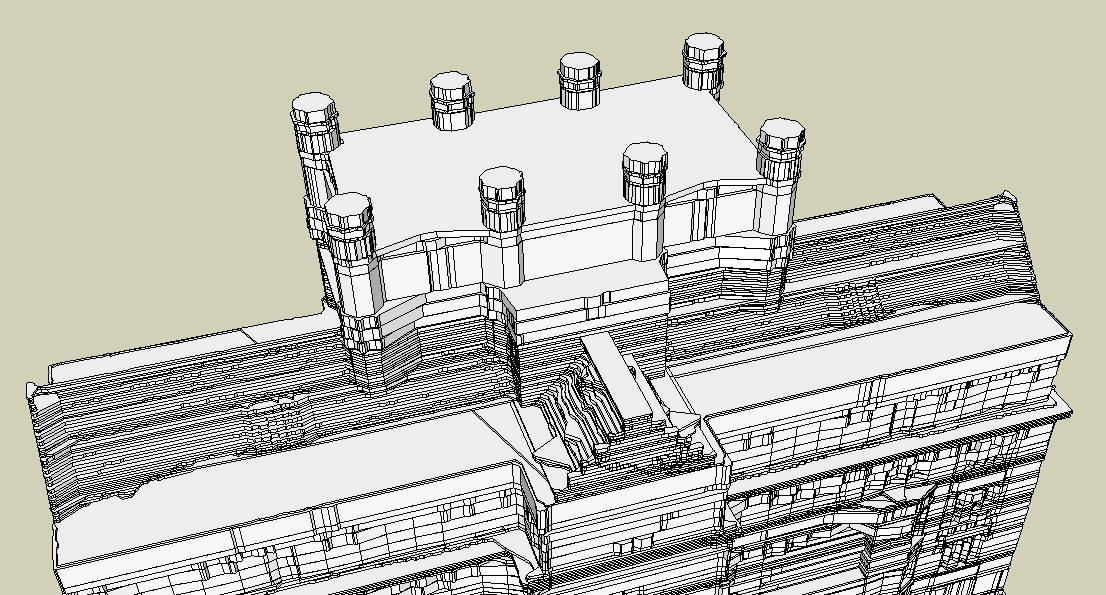
\includegraphics[width=0.22\textwidth]{extrude_1.png} &
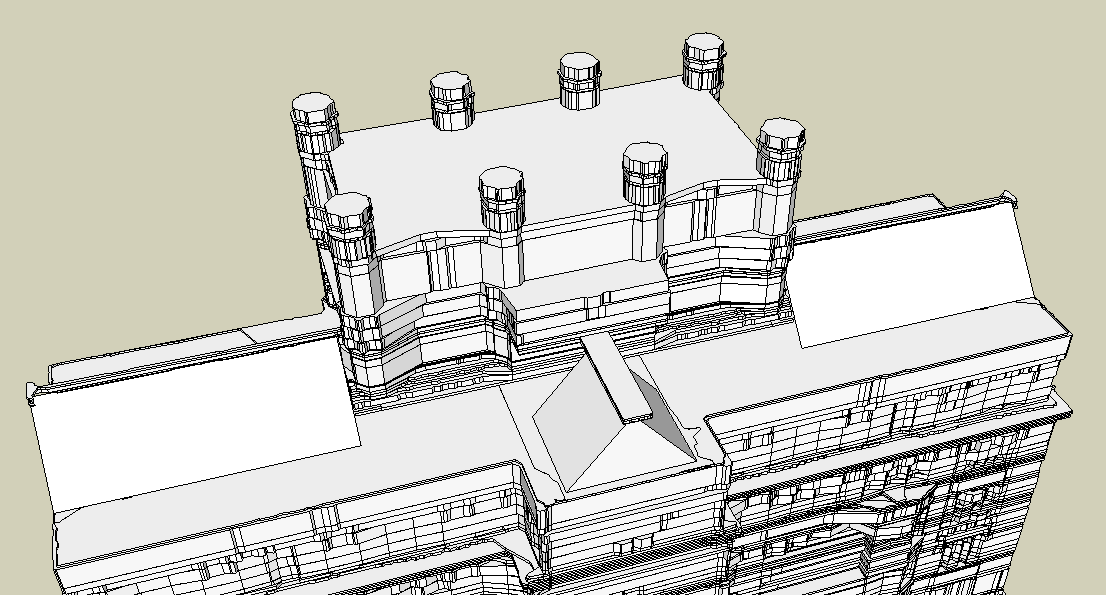
\includegraphics[width=0.22\textwidth]{extrude_2.png} \\
(a) & (b)
\end{tabular}
\end{center}
\caption{The top view of the 3D building shown 
(a) without tapered structures
and (b) with tapered structures.}
\label{fig:DXF_top}
\end{figure}

The difficulty in inferring tapered structures is tied to 
the complexity of a building structure itself.
Fortunately, the dataset segmentation module introduced in \Sec{mseg} 
has segmented the complicated structures into simpler parts.
%The majority of tapered structures in a building are due to
%{\it linear tapering}.
%This includes cone-shape geometry due to a {\it taper to point} (TTP)
%operation, as illustrated in \Figa{taper_cases}, and
%wedge-shape geometry due to a {\it taper to line} (TTL) operation,
%as shown in \Figb{taper_cases}.
%Tapered structures may also include dome-shape geometry due to complicated
%{\it non-linear tapering} operations, as depicted in \Figc{taper_cases}.
%Furthermore, a structure may look like a tapered structure, 
%but it is actually not a real one.
%For example, a series of small extruded structures 
%form a tapered-like shape in \Figd{taper_cases}.
Although the majority of building tapering structures are {\it linear tapering},
such as {\it tapering to point} (TTP), a cone shape geometry,
and {\it tapering to line} (TTL), a wedge shape,
it could also be a complicated {\it non-linear tapering},
such as a dome shape.
Furthermore, a structure may look like a tapering structure,
but it is actually not a real one.
For example, a series of small extruded structures
form a tapering-like shape.

We introduced a two-step workflow to accomplish the above goal.
The first step is to locate the potential tapering keyslices
and infer the structure by making an assumption that
the underlying tapering structure is either a TTP or a TTL.
A verification step is conducted to check the correctness
of the inferred shape by measuring the error between the model and
the corresponding 3D PCD.
If the error is small, the inferred shape is confirmed
and the underlying keyslices are not rendered.
Otherwise, we can choose to model this special structure by fitting a
triangular mesh to the underlying 3D point cloud to produce a polygonal model.
This algorithm cannot model a sphere or a dome because such structure
cannot be linearly interpolated as a taper operation.

% We first check whether it is necessary to do taper detection by
% examining the keyslices computed from all major sweeping directions. 
% If the segment under analysis can be interpreted by a few keyslices
% from certain sweeping directions, we mark this segment as an extruded
% structure and therefore skip the taper detection for it.
% Otherwise, taper detection will be conducted in the standard bottom-up direction.
% 
% We introduced a two-step workflow to accomplish taper detection.
% The first step is to locate the potential tapered keyslices
% and infer the structure by making an assumption that 
% the underlying tapered structure is either a TTP or a TTL.
% Then a verification step is carried out to check the correctness 
% of the inferred shape by measuring the error between the model and
% the corresponding 3D PCD.
% If the error is small, the inferred shape is confirmed
% and the underlying keyslices are not rendered.
% Otherwise, we can choose to model this special structure by fitting a
% triangular mesh to the underlying 3D point cloud to produce a polygonal model.
% This algorithm cannot model a sphere or a dome because such structures
% cannot be linearly interpolated as a taper operation.
% 
% \begin{figure}[htbp]
% \begin{center}
% \begin{tabular}{cc}
% 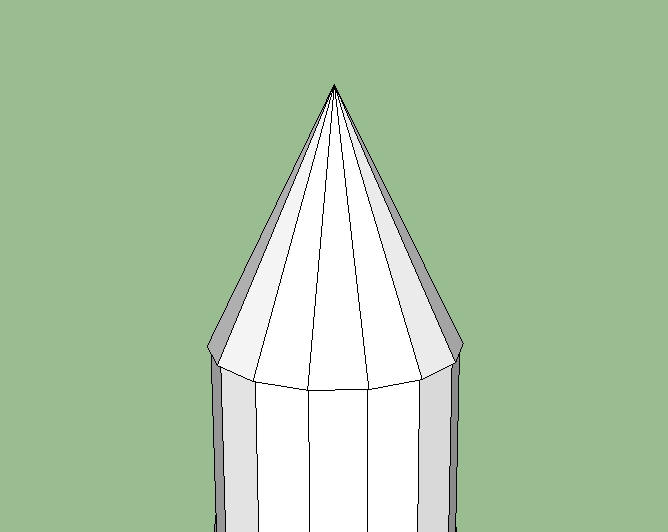
\includegraphics[width=0.18\textwidth]{tapering_case1.png} &
% 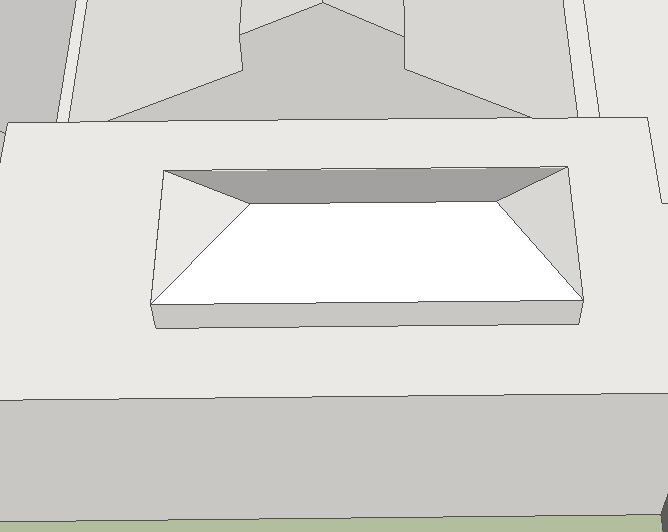
\includegraphics[width=0.18\textwidth]{tapering_case2.png} \\
% (a) & (b) \\
% 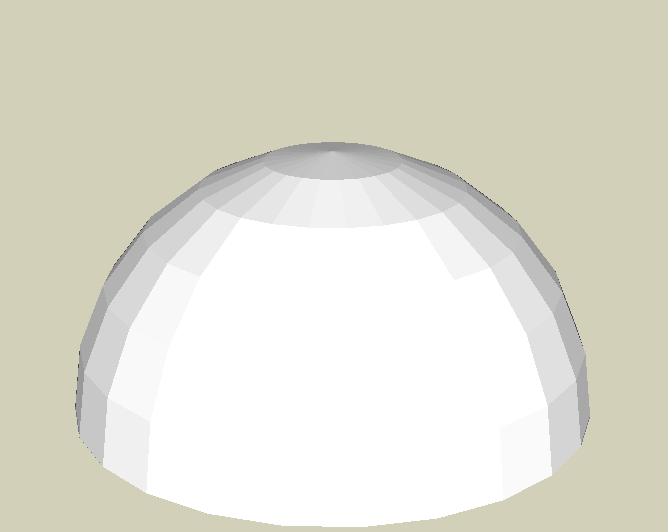
\includegraphics[width=0.18\textwidth]{tapering_case3.png} &
% 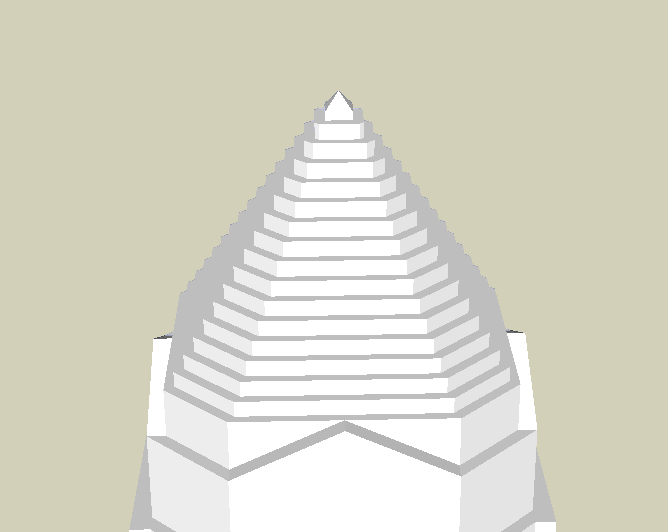
\includegraphics[width=0.18\textwidth]{tapering_case4.png} \\
% (c) & (d) 
% \end{tabular}
% \end{center}
% \caption{The component of (a) tapering to a point (b) tapering to a line 
% (c) non-linear tapering (d) non-tapered structures. }
% \label{fig:taper_cases}
% \end{figure}
% 
The assumption of linear tapering to a line or point makes inferring
tapered structures much simpler and more efficient. 
For a keyslice set ${\bf N_K} = \{I_i | 0 \le i \le N \}$, 
where $i$ is the projected slice index, we first compute
the sets of keyslices for potential tapered structures.
This is based on the observation that for tapering structures,
the underlying keyslices indices form nearly an arithmetic progression. 
The keyslice set ${\bf N_T}$ indicates a potential section of a
tapered structure in the projected range.
${\bf N_T}$ also provides a very important information for inferring the
underlying structure: based on the assumption, the first element, $I_0$,
in ${\bf N_T}$ is the base geometry shape for the linear tapered structure.
And the last element, $I_f$, of ${\bf N_T}$ 
is the converged or partially converged geometry shape.
If $I_f$ contains either a line segment or a point structure,
this indicates that the underlying tapered structure of ${\bf N_T}$
is completely converged.

\begin{figure}[htbp]
\begin{center}
\begin{tabular}{cc}
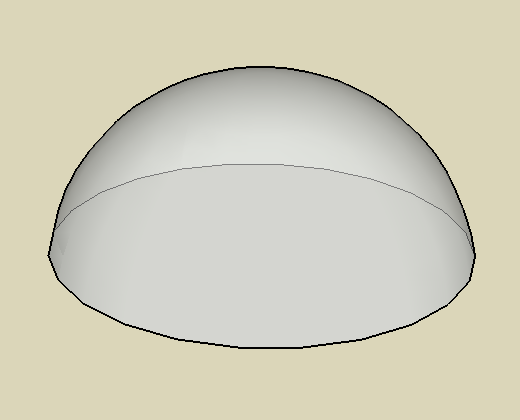
\includegraphics[width=0.2\textwidth]{taper_dome_0.png} &
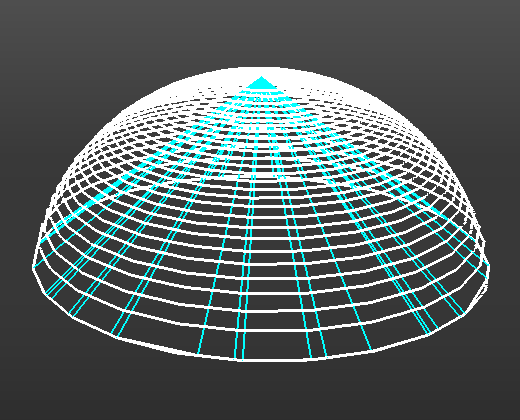
\includegraphics[width=0.2\textwidth]{taper_dome_4.png} \\
(a) & (b)
\end{tabular}
\end{center}
\caption{The verification of the inferred tapered structure:
(a) the original model;
(b) the computed keyslices (in white) and inferred tapering to point structure (in blue).
}
\label{fig:taper_taper_dome}
\end{figure}

The basic idea for the verification stage is to measure the error 
for the new inferred tapered structure. 
The error is defined as the distance $d_e$ between a 3D point $p$ and 
the inferred model $M$.
If $d_e$ is smaller than a threshold, $t$, the tapered structure is approved and 
the corresponding keyslices are substituted to further compress the model.
Otherwise, the underlying tapered structure is rejected,
and we can choose to model this special structure by its keyslices or
by fitting a triangular mesh to the underlying 3D point cloud
to produce a polygonal model.
\Fig{taper_taper_dome} shows a dome model which was first modeled
as a taper to a point structure (in blue)
but later on was rejected by the verification process.
We chose $t = \tau_d/2$ as the threshold, 
and it worked well on our synthetic and real datasets.
Here, $\tau_d$ is the threshold for keyslice detection 
as introduced in \Sec{ksd}.

%%%%%%%%%%%%%%%%%%%%%%%%%%%%%%%%
%%%%%%   Model Reconstruction  %
%%%%%%%%%%%%%%%%%%%%%%%%%%%%%%%%
\section{Model Generation}
To generate the final 3D model, the control
points of the 2D contours can be transformed back into 3D world coordinate system
using the reverse matrix $T$ in equation \Eq{image_slicing}.
For each segment, we first exam whether it can be modeled 
by simple keyslices along any major plane.
If so, the push-pull operation is applied to the keyslice contours to
generate the extruded model.
If a tapered structure is detected, we construct the faces
based on the control points of the 2D base geometry polygon 
and their corresponding converged points to create the tapered model.

\subsection{Model Merging}

The reconstruction becomes more complicated when multiple segments 
need to be assembled since some segments may share the same vertices or edges. 
Therefore model merging needs to be done
for the reconstruction of the whole final model.

\begin{figure}[htbp]
  \centering
  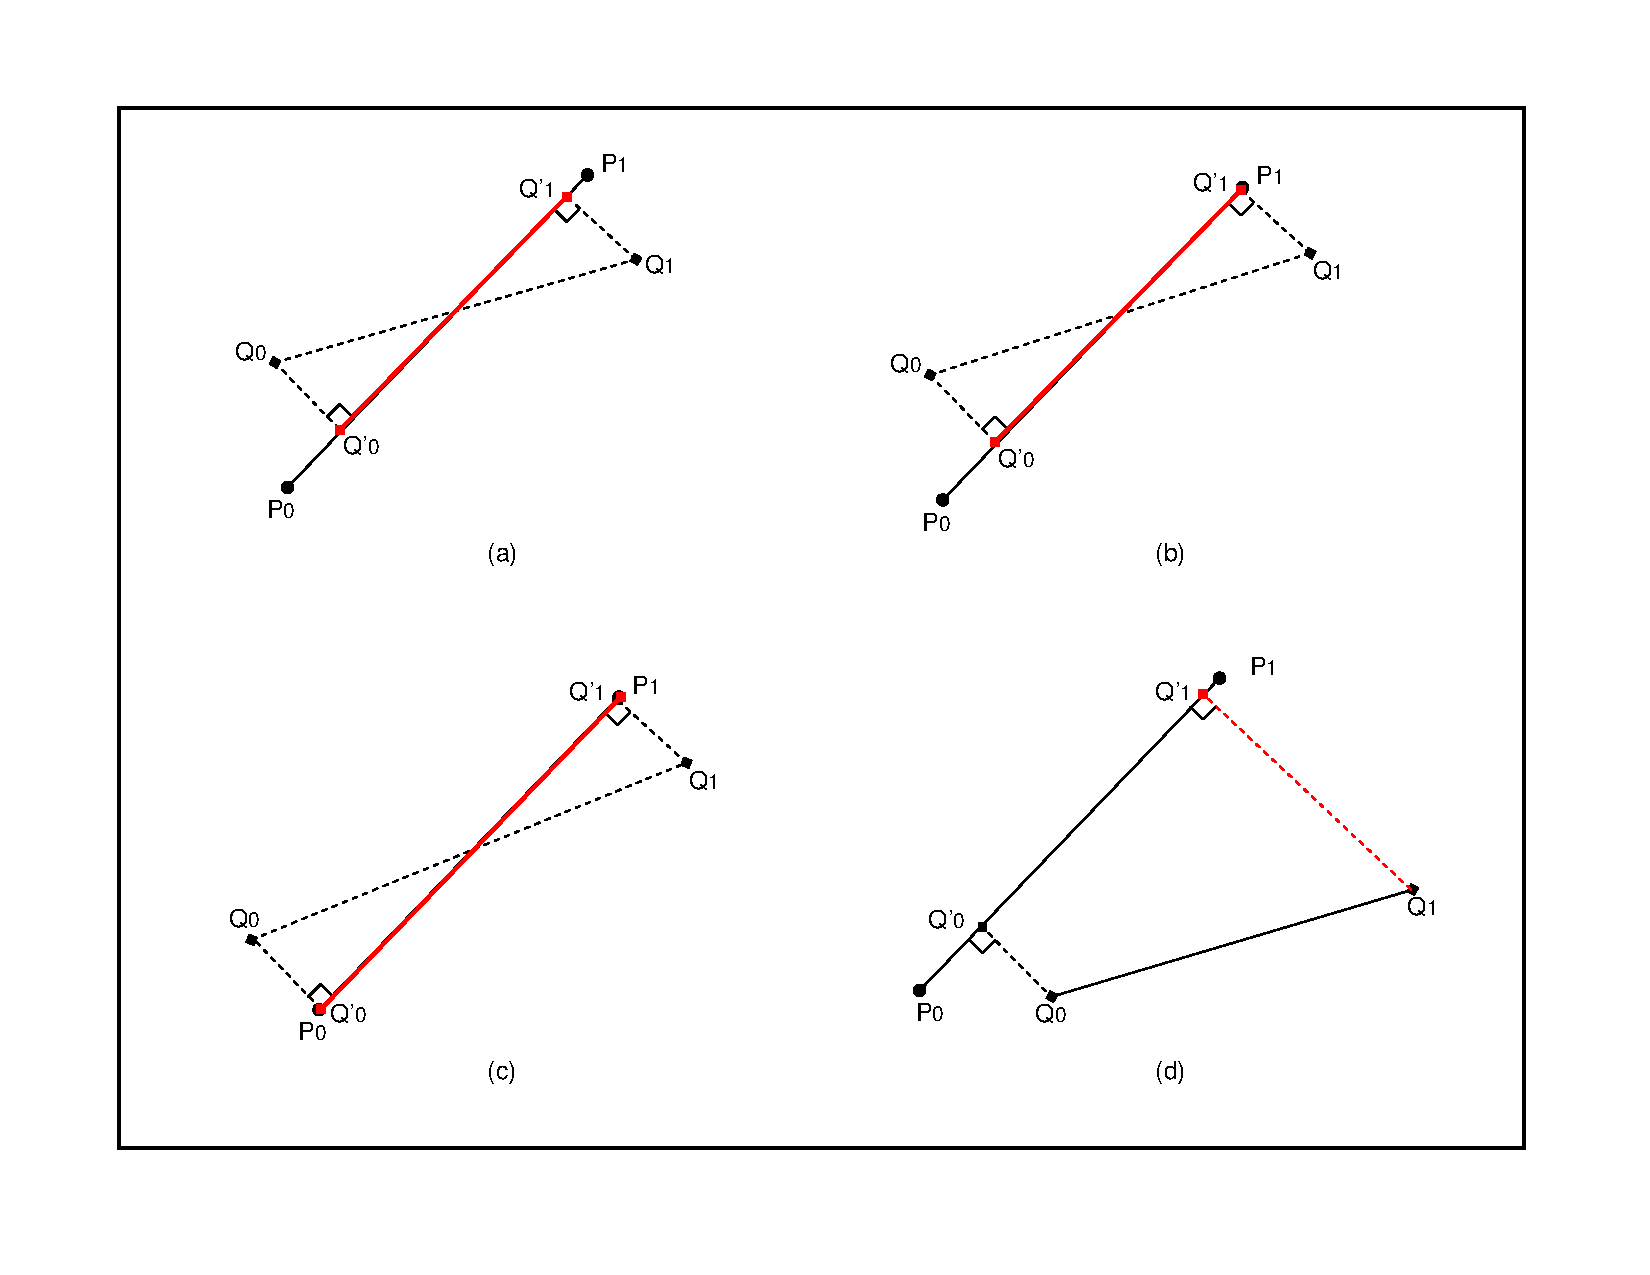
\includegraphics
      [width=0.35\textwidth]
      {model_merge.pdf}
      \caption{Vertices adjustment for model merging
      (a) the two new points $Q_0$ and $Q_1$ are projected to 
          an existed line as $Q'_0$ and $Q'_1$.
      (b) after (a), $Q'_1$ is merged with an existed point $P_1$.
      (c) after (a), both $Q'_0$ and $Q'_1$ are merged with 
          existed point $P_0$ and $P_1$ respectively.
      (d) one of the point $Q_1$ is too far away for adjustment. }
      \label{fig:MR_Fig1}
\end{figure}

The first segmented part can be easily reconstructed without merging. 
Let ${\bf M}$ represent all lines or planes added into the final model so far. 
When adding a new line segment $Q_0Q_1$ to the model, 
we need to compute the closest line ${\bf L} = P_0P_1$ in ${\bf M}$ to $Q_0Q_1$.
Let $d = max(dist(Q_0, {\bf L}), dist(Q_1, {\bf L}))$, i.e., the larger distance 
between $Q_0$ to ${\bf L}$ and $Q_1$ to ${\bf L}$.
The distance from a point $Q$ to a line ${\bf L}$ can be computed using the equation:
\begin{equation*} % point to line equation
d(Q, { \bf L}) = | {\bf w - (w \cdot u) \, u} |
\end{equation*}
where ${\bf w} = (Q - P_0) $ and {\bf u} is the unit direction vector of {\bf L}.

There are several cases to be considered.
If $d <= \delta$, that is, both $Q_0$ and $Q_1$ are close enough to $L$, 
the projected point $Q'_0$ and $Q'_1$
are used to replace $Q_0$ and $Q_1$ respectively as shown in \Figa{MR_Fig1}. 
Furthermore, if one of the projected point, 
say $Q'_1$ is close to an end point of $L$, say $P_1$, 
$Q'_1$ would be merged with $P_1$ as shown in \Figb{MR_Fig1}. 
If both $Q'_0$ and $Q'_1$ are matched with $P_0$ and $P_1$, 
the line $Q_0Q_1$ would be merged totally with the line $L$, 
which was shown in \Figc{MR_Fig1}.
However, if $d > \delta$, no merging should be conducted as shown in \Figd{MR_Fig1}. 
\Figa{MR_Fig2} and \Figb{MR_Fig2} show the structures before and after model merge.


\begin{figure} [htbp]
\begin{center}
\begin{tabular}{cc}
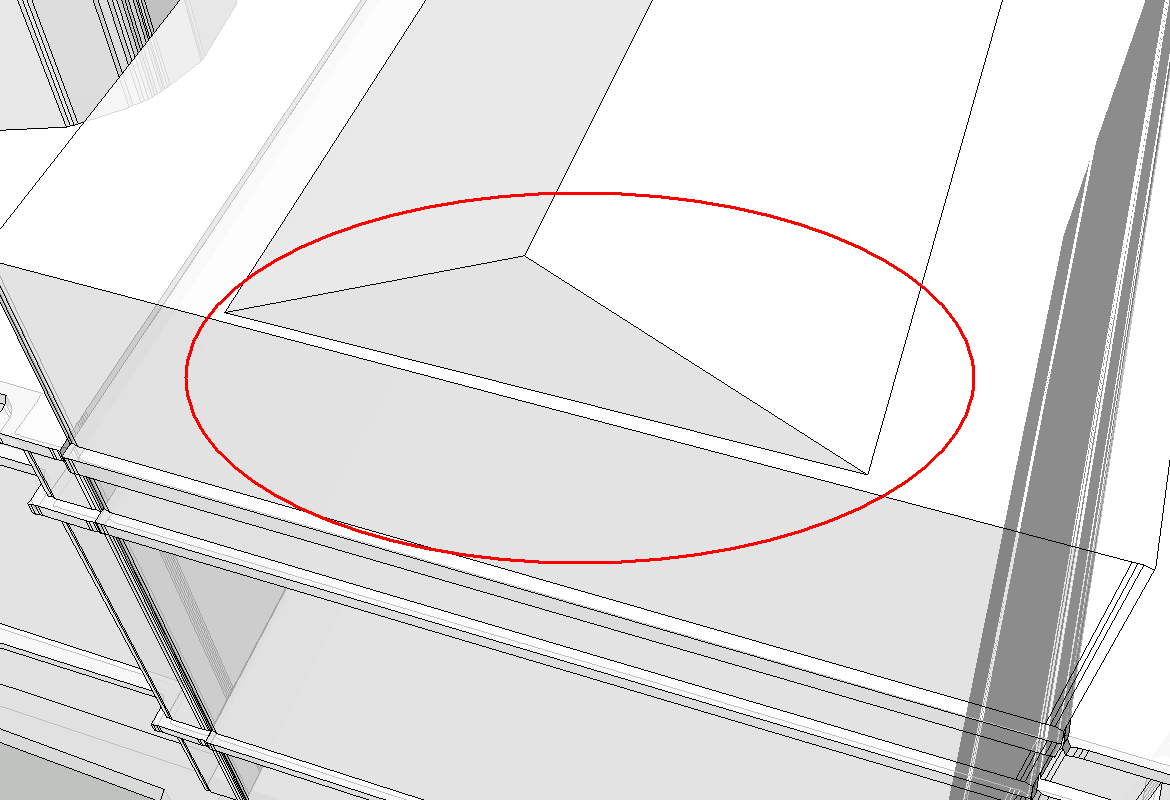
\includegraphics[width=0.22\textwidth]{model_before_merge.png} &
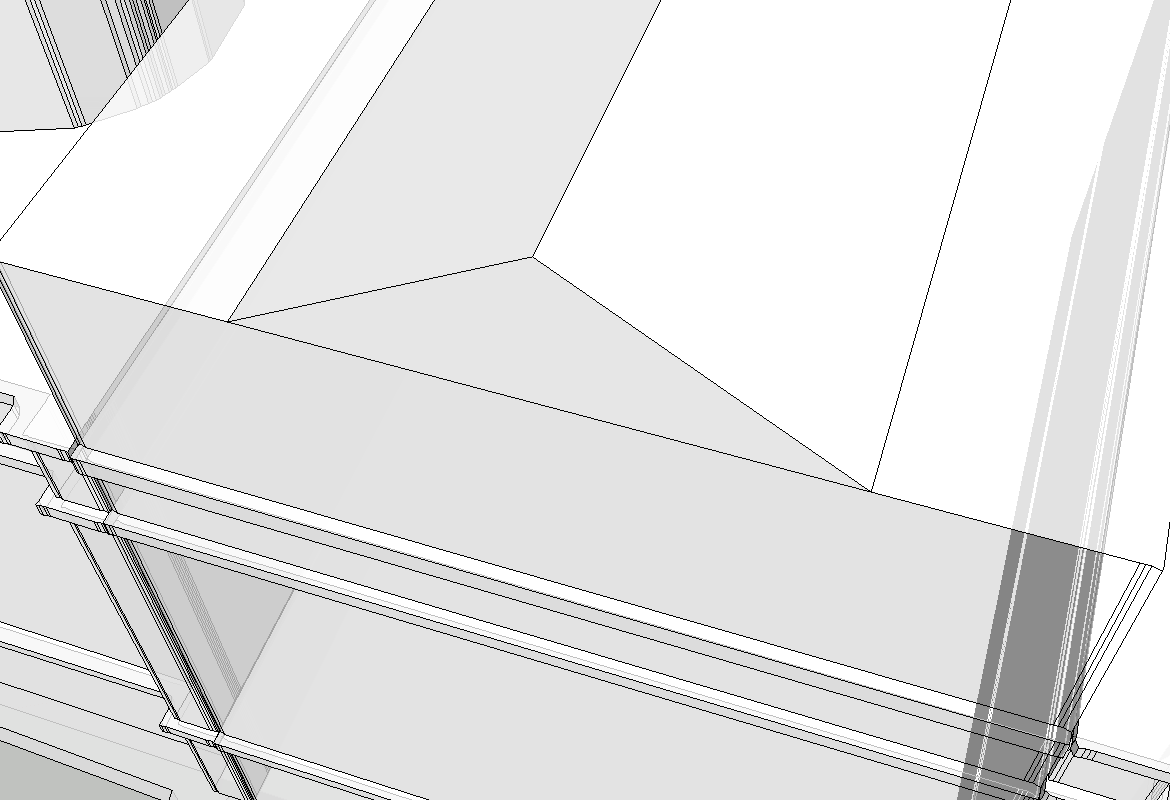
\includegraphics[width=0.22\textwidth]{model_after_merge.png} \\
(a) & (b) 
\end{tabular}
\end{center}
\caption{ 
      (a) two structures inside red ellipse are separated before merge
      (b) new structures after merge}
\label{fig:MR_Fig2}
\end{figure}

\subsection{Window Installation}

After the model merging, the whole reconstructed model has been generated. 
We call this {\it naked} model in that there is no windows or doors yet 
as shown in \Figa{WDR_Fig1}.
If the point cloud contains windows or doors, 
we need to add them onto the naked model.
The window and door structures have been computed in \Sec{wdd}.
The idea is to find the closest face, $F_{win}$, in the final model
for a window $w$ to be added.
To add $w$ on $F_{win}$, we only need to compute the projected point $P'$ 
for each vertex $P$ in $w$ onto $F_{win}$.
A simple push-pull operation on $F_w$ with the distance of window depth
will add the window $w$ onto $F_w$ of the naked model.
\Figb{WDR_Fig1} shows the entire model 
with windows and doors added for the model in \Figa{WDR_Fig1}.

\begin{figure} [htbp]
\begin{center}
\begin{tabular}{cc}
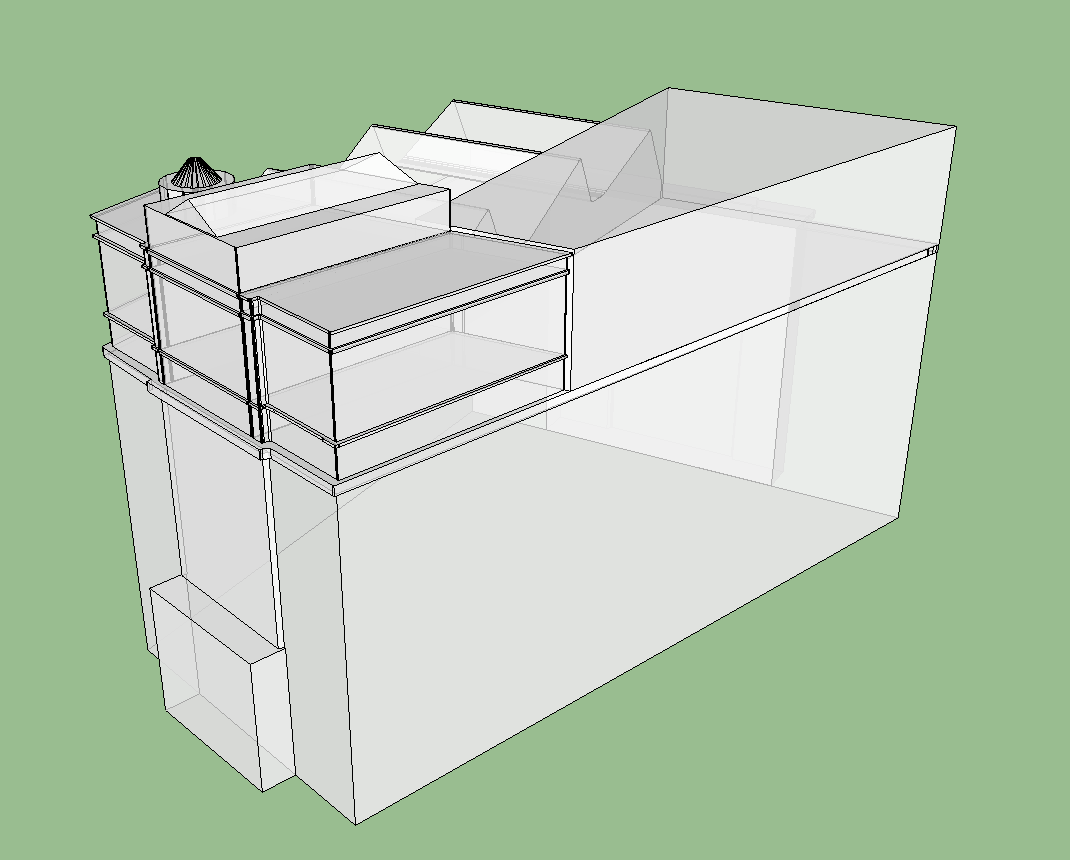
\includegraphics[width=0.22\textwidth]{model_naked.png} &
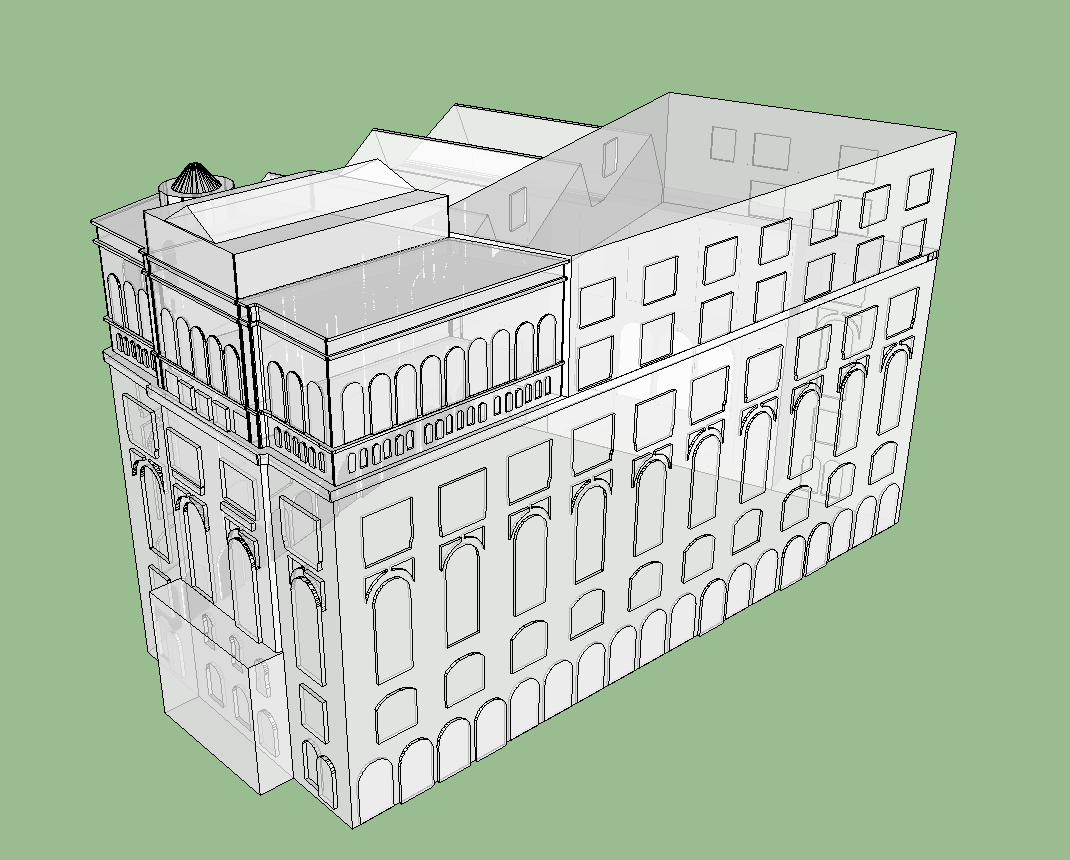
\includegraphics[width=0.22\textwidth]{model_windows.png} \\
(a) & (b) 
\end{tabular}
\end{center}
\caption{ Windows and doors reconstruction:
      (a) the reconstructed naked model.
      (b) the whole model with windows and doors added.}
\label{fig:WDR_Fig1}
\end{figure}


%%%%%%%%%%%%%%%%%%%%%%%%%%%%%%%%
%%%%%%   Experimental Results%%%
%%%%%%%%%%%%%%%%%%%%%%%%%%%%%%%%
\section{Experimental Results}
\label{sec:IR_OUT}

\Fig{results} shows the experimental results for both synthetic and 
real datasets (in the last two rows).
Each row shows a reconstruction of a building. 
The snapshot of the original model or the image of the real building
is shown in (a), followed by the snapshot of 3D PCD in (b).
Columns (c)-(e) respectively depict the segmentation result,
the vectorized keyslices, and the snapshot of the extruded model.
If the model tapers to a point or contains windows, 
the updated final model is shown in (f).

\begin{figure*}[htbp]
\begin{center}
\begin{tabular}{cccccc}
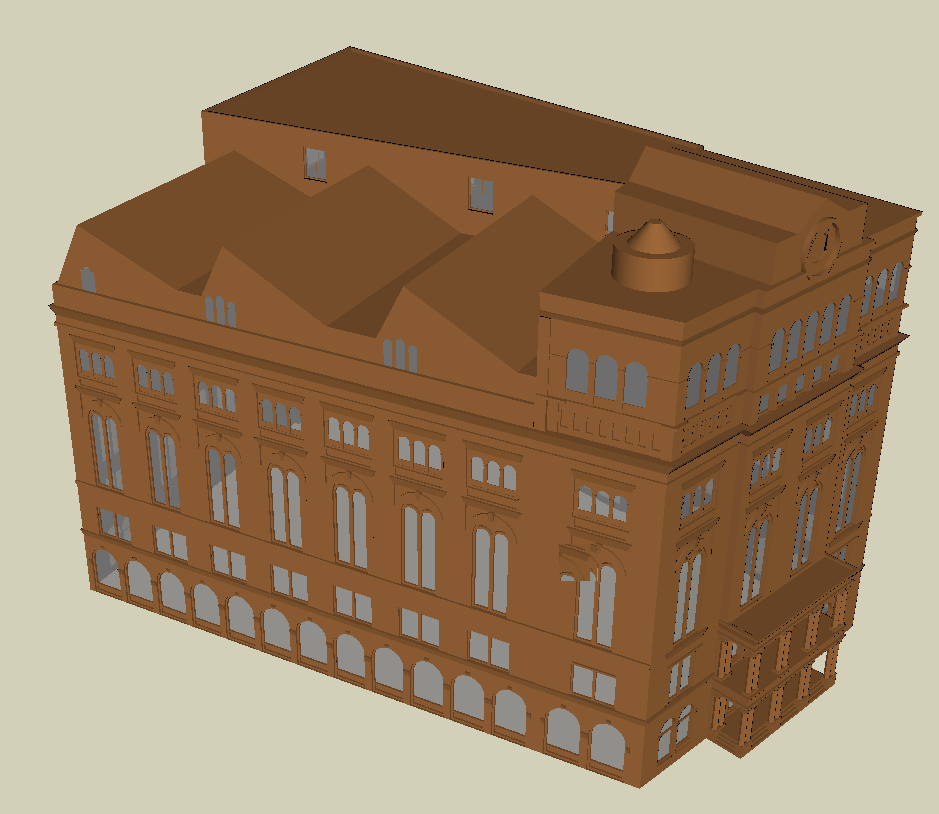
\includegraphics[width=0.15\textwidth]{cu_1.png} &
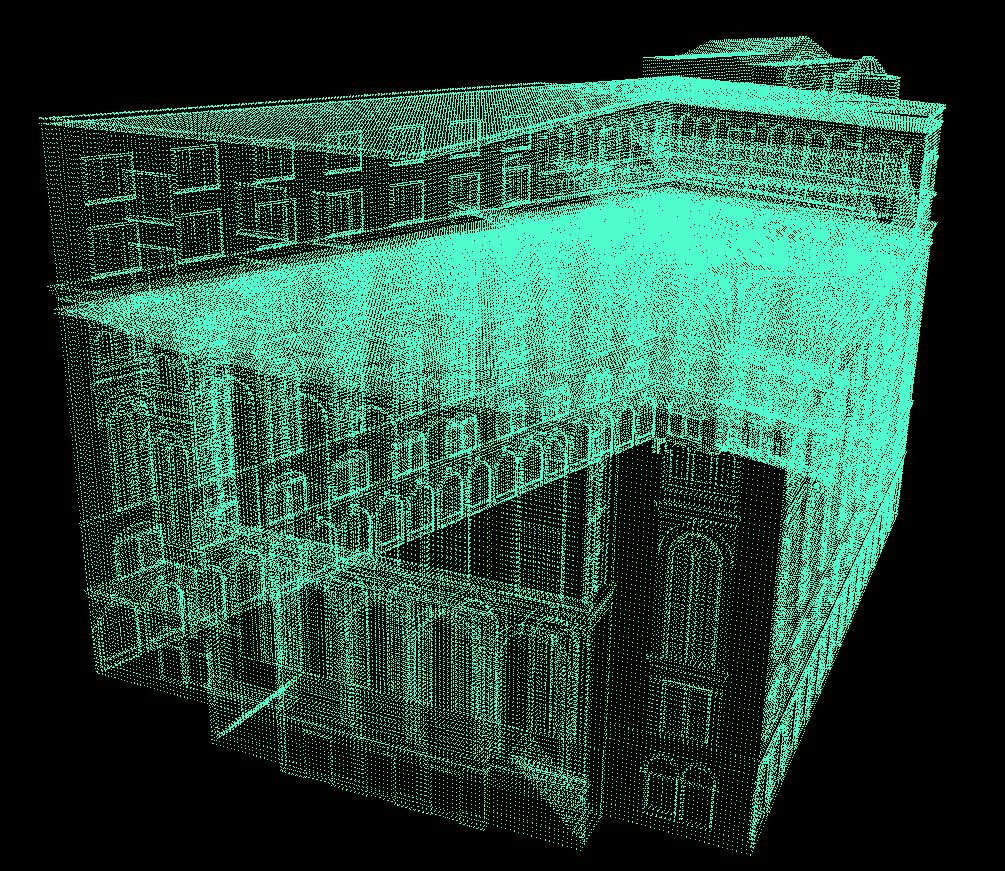
\includegraphics[width=0.15\textwidth]{cu_2.png} &
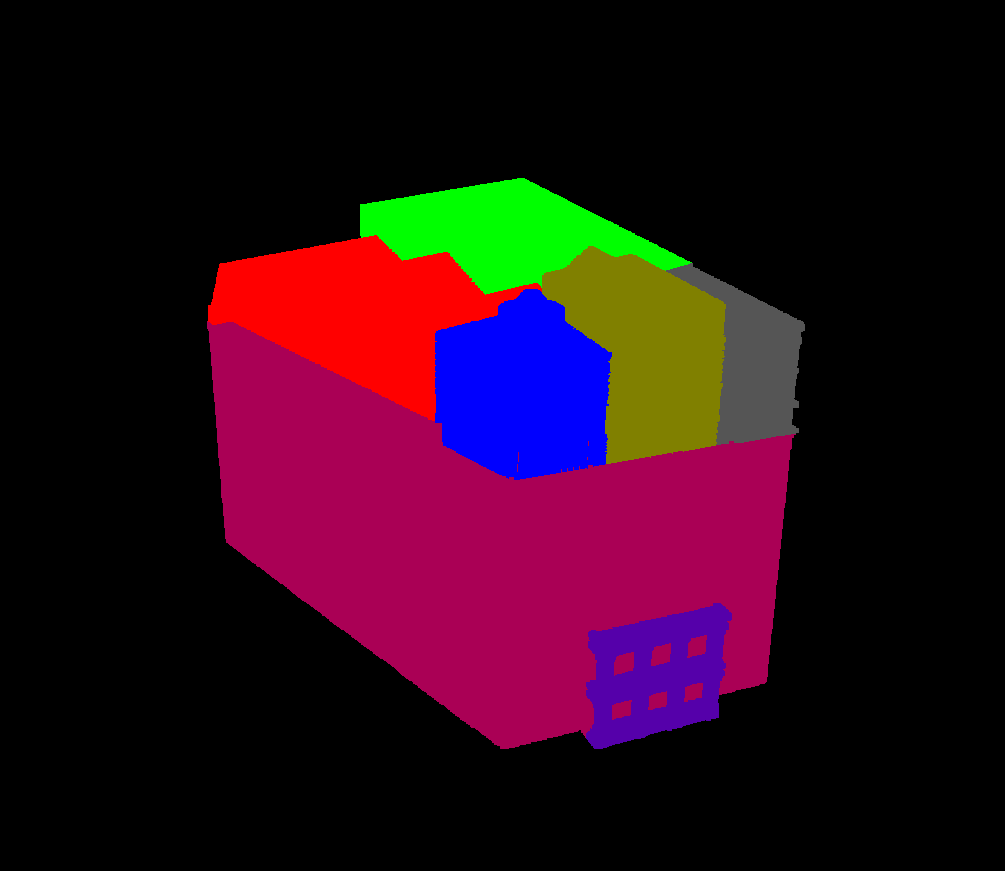
\includegraphics[width=0.15\textwidth]{cu_7.png} &
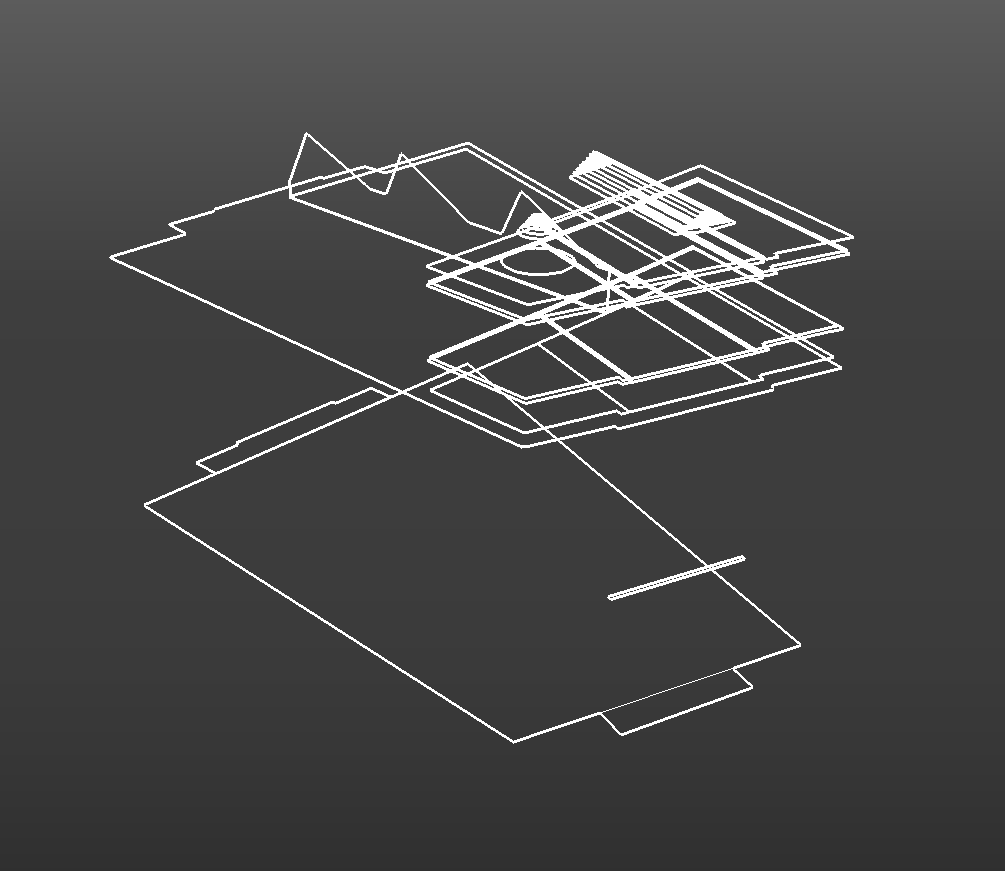
\includegraphics[width=0.15\textwidth]{cu_9.png} &
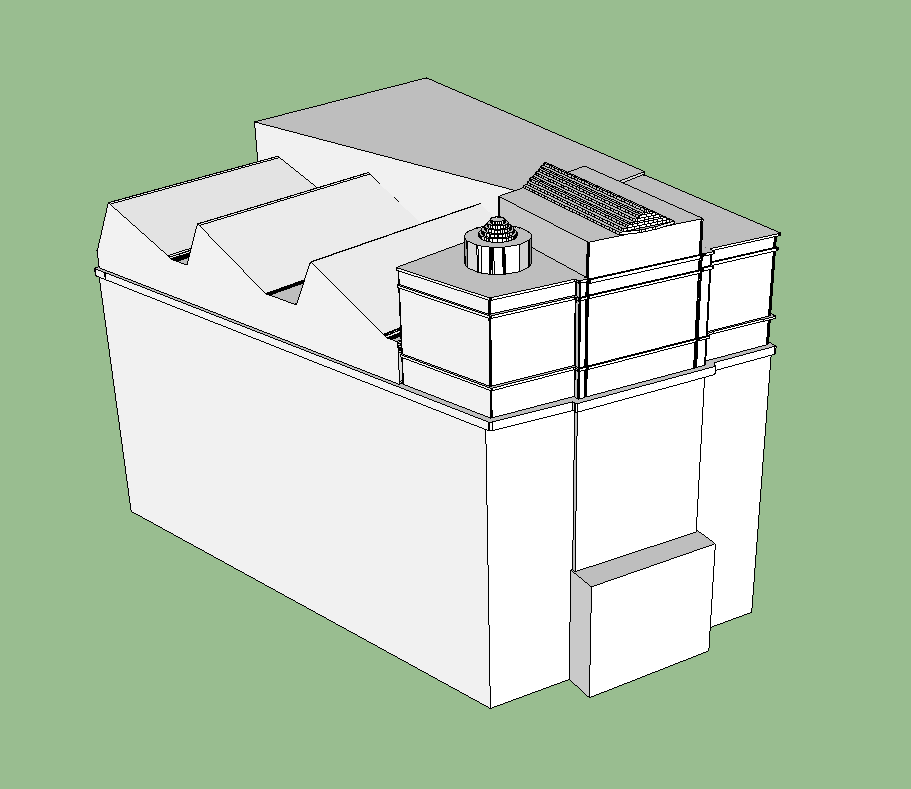
\includegraphics[width=0.15\textwidth]{cu_11.png} &
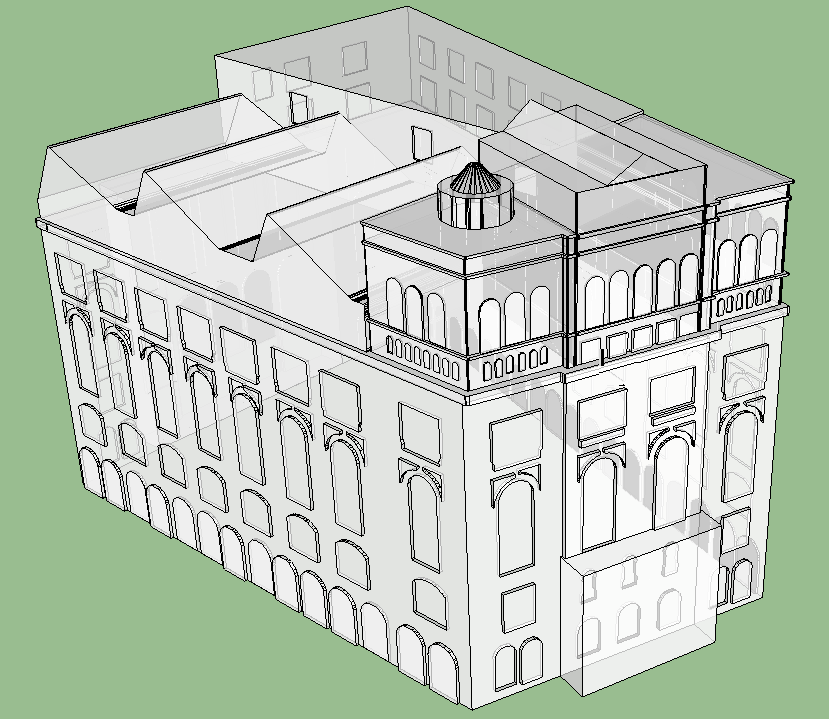
\includegraphics[width=0.15\textwidth]{cu_3.png} \\
% (a) & (b) & (c) & (d) & (e) & (f) \\
\includegraphics[width=0.15\textwidth]{health_town_1.png} &
\includegraphics[width=0.15\textwidth]{health_town_2.png} &
\includegraphics[width=0.15\textwidth]{health_town_7.png} &
\includegraphics[width=0.15\textwidth]{health_town_9.png} &
\includegraphics[width=0.15\textwidth]{health_town_11.png} &
\includegraphics[width=0.15\textwidth]{health_town_3.png} \\
% (a) & (b) & (c) & (d) & (e) & (f) \\
\includegraphics[width=0.15\textwidth]{spitak_1.png} &
\includegraphics[width=0.15\textwidth]{spitak_2.png} &
\includegraphics[width=0.15\textwidth]{spitak_7.png} &
\includegraphics[width=0.15\textwidth]{spitak_9.png} &
\includegraphics[width=0.15\textwidth]{spitak_11.png} &
\includegraphics[width=0.15\textwidth]{spitak_3.png} \\
% (a) & (b) & (c) & (d) & (e) & (f) \\
%\includegraphics[width=0.15\textwidth]{branch_lib_1.png} &
%\includegraphics[width=0.15\textwidth]{branch_lib_2.png} &
%\includegraphics[width=0.15\textwidth]{branch_lib_7.png} &
%\includegraphics[width=0.15\textwidth]{branch_lib_9.png} &
%\includegraphics[width=0.15\textwidth]{branch_lib_11.png} &
%\includegraphics[width=0.15\textwidth]{branch_lib_3.png} \\
% (a) & (b) & (c) & (d) & (e) & (f) \\
\includegraphics[width=0.15\textwidth]{doe_1.png} &
\includegraphics[width=0.15\textwidth]{doe_2.png} &
\includegraphics[width=0.15\textwidth]{doe_7.png} &
\includegraphics[width=0.15\textwidth]{doe_9.png} &
\includegraphics[width=0.15\textwidth]{doe_11.png} &
\includegraphics[width=0.15\textwidth]{doe_3.png} \\
% (a) & (b) & (c) & (d) & (e) & (f) \\
\includegraphics[width=0.15\textwidth]{GCT_1.jpg} &
\includegraphics[width=0.15\textwidth]{GCT_2.png} &
\includegraphics[width=0.15\textwidth]{GCT_7.png} &
\includegraphics[width=0.15\textwidth]{GCT_9.png} &
\includegraphics[width=0.15\textwidth]{GCT_10.png} &
\includegraphics[width=0.15\textwidth]{GCT_3.png} \\
% (a) & (b) & (c) & (d) & (e) \\
\includegraphics[width=0.15\textwidth]{HunterPhoto.jpg} &
\includegraphics[width=0.15\textwidth]{point_cloud.png} &
\includegraphics[width=0.15\textwidth]{TH_7.png} &
\includegraphics[width=0.15\textwidth]{TH_9.png} &
\includegraphics[width=0.15\textwidth]{TH_10.png} &
\includegraphics[width=0.15\textwidth]{TH_3.png} \\
% (a) & (b) & (c) & (d) & (e) \\
\includegraphics[width=0.15\textwidth]{real_cu_1.jpg} &
\includegraphics[width=0.15\textwidth]{real_cu_2.png} &
\includegraphics[width=0.15\textwidth]{real_cu_7.png} &
\includegraphics[width=0.15\textwidth]{real_cu_9.png} &
\includegraphics[width=0.15\textwidth]{real_cu_10.png} &
\includegraphics[width=0.15\textwidth]{real_cu_3.png} \\
% (a) & (b) & (c) & (d) & (e) \\
\includegraphics[width=0.15\textwidth]{opernhaus_1.png} &
\includegraphics[width=0.15\textwidth]{opernhaus_2.png} &
\includegraphics[width=0.15\textwidth]{opernhaus_3.png} &
\includegraphics[width=0.15\textwidth]{opernhaus_4.png} &
\includegraphics[width=0.15\textwidth]{opernhaus_5.png} &
\includegraphics[width=0.15\textwidth]{opernhaus_6.png} \\
(a) & (b) & (c) & (d) & (e) & (f)
\end{tabular}
\end{center}
\caption{The experimental results. The snapshot of 
(a) original model / picture, 
(b) 3D point cloud of (a),
(c) the segmentation,
(d) the keyslices,
(e) the extrusion model,
(f) the enhanced model of (e) with tapered and window installed.
The data of the Opernhaus Hannover in the bottom row is provided courtesy of 
the Institute of Cartography and Geoinformatics, University of Hannover.
}
\label{fig:results}
\end{figure*}

%\section{Performance Evaluation}
%
To measure the error of a reconstructed 3D model, we first transform it
to the 3D point cloud coordinate system.
The error $E$ is measured as the distance between the 3D points in the cloud
to their closest planes in the reconstructed model $M$:
\begin{equation}
E = \frac{1}{|X|}\sum_{x\in{X}}{d(x, M)}
\label{eq:em}
\end{equation}
where $X$ is the set of 3D points, and distance
$d(x, M) = \text{min}_{p \in M}\lVert x - p \lVert$ is the minimum
Euclidean distance from a 3D point $x$ to its closest face $p$ of $M$.

\begin{figure} [htbp]
\begin{center}
\begin{tabular}{cc}
\includegraphics[width=0.24\textwidth]{error_1000_32_4.png} &
\includegraphics[width=0.24\textwidth]{error_1000_4_1.png} \\
(a) & (b)
\end{tabular}
\end{center}
\caption{The deviation map of the 3D point cloud. 
(a) The result with $\tau_r$ = 4 and $\tau_d$ = 32.
(b) The result with $\tau_r$ = 1 and $\tau_d$ = 4. }
\label{fig:EM}
\end{figure}

To visualize the error between real 3D data and the inferred model,
we generate deviation map images.
Two such images are shown in \Fig{EM} for the PCD in
\Figb{IR_2_DXF}.
The deviation maps are constructed as follows.
For each face $p$ of $M$, a corresponding texture image is computed.
The intensity of each pixel in the texture image is determined by the error
of the corresponding 3D points computed by \Eq{em}.
The accuracy of the reconstructed model is controlled by Hausdorff distance
threshold $\tau_d$ and BPA refinement radius $\tau_r$.
Threshold $\tau_d$ determines the accuracy of keyslice detection and $\tau_r$
determines the accuracy of boundary vectorization.

\Tbl{em} lists the relationship among the $\tau_d$, errors,
number of faces, and model size for the input data in \Figb{IR_2_DXF}.
The unit for $\tau_d$ is in pixels and the unit for error is in meters.
The size of the original point cloud for the 3D building is more than 700 MB.
From the table, we can see that even for the most accurate model, 
the size is dramatically reduced compared with the original 3D PCD.
This is a desirable property for web-based applications.
The low resolution ($\tau_d = 64$) and high resolution ($\tau_d = 4$) models
were generated in 15 and 120 minutes, respectively,
on a laptop PC using an Intel Core 2 T7200 CPU at 2.0 GHz with 2.0 GB RAM.
Future work includes the optimization of the BPA vectorization module since
it consumes approximately 70\% of the computation time.

%\setlength{\tabcolsep}{4pt}
\begin{table}[hbtp]
\begin{center}
\begin{tabular}[t]{||c||c|c|c|c||}
\hline
$\tau_d $(pixel) & Error (m)& \# of faces & Size (KB) & time (s) \\ \hline \hline
64 & .658 $\pm$ .158 & 1471  & 15  & 1977 \\ \hline 
32 & .294 $\pm$ .103 & 3284  & 32  & 2353 \\ \hline
16 & .141 $\pm$ .058 & 8574  & 86  & 3008 \\ \hline
8  & .131 $\pm$ .074 & 13955 & 137 & 3696 \\ \hline
4  & .094 $\pm$ .068 & 27214 & 261 & 5391 \\ \hline
2  & .088 $\pm$ .036 & 31331 & 335 & 7586 \\ \hline
1  & .083 $\pm$ .041 & 32187 & 337 & 10927\\ \hline
\end{tabular}
\end{center}
\caption{Error measurements for reconstruction of Thomas Hunter with $\tau_r = 4$.}
\label{tbl:em}
\end{table}
%\setlength{\tabcolsep}{1.4pt}

\subsection{Model Comparison}

Although models generated by 3D BPA are of high resolution, they usually
require excessive storage capacity.
The model in \Fig{TH_BPA}, for example, needs almost 400 MB of storage,
which prevents this solution from being applied to web-based applications.
One way to improve matters is to apply some approximation/decimation
technique to reduce the space required by these models.

The holes in the 3D BPA model in \Fig{TH_BPA} are present in the
original dataset.
They are due to the fact that the laser never reflected back to
the scanner after penetrating the glass windows.
The 3D BPA method is deficient in filling these holes.
We counter this problem by first applying a symmetry-based hole filling
algorithm on the 2D slices to create enhanced slices that are processed
by an adaptive 2D BPA method to fill gaps.
Finally, an extrusion operation is applied to create a watertight 3D model.
\begin{figure}[htbp]
\begin{center} 
\begin{tabular}{cc}
\includegraphics[width=.22\textwidth]{BPA_TH.png} &
\includegraphics[width=.22\textwidth]{BPA_TH_1.png}
\end{tabular}
\end{center}
\caption{Dense triangulated BPA mesh cropped from \Figb{IR_2_DXF}.}
\label{fig:TH_BPA}
\end{figure}
Among all mesh reduction techniques, {\it qslim} is one of the most
sophisticated and efficient algorithms \cite{BPA_GH}.
We carried out a comparison between models generated by our proposed
method and those approximated by {\it qslim}.
The comparisons were conducted on models sharing the same number of faces.
It is worth noting that {\it qslim} ran out of memory on the 3D model data
generated by BPA in \Fig{TH_BPA}.
To reduce the size of the model for {\it qslim} to work, we had
to either downsample the 3D model generated by BPA or split it into
sub-models which can be handled by {\it qslim}.

\begin{figure}[htbp]
\begin{center}
\begin{tabular}{cc}
\includegraphics[width=0.22\textwidth]{comp_32_2_qslim.png} &
\includegraphics[width=0.22\textwidth]{comp_4_2_qslim.png} \\
(a) & (b) \\
\includegraphics[width=0.22\textwidth]{comp_32_2.png} &
\includegraphics[width=0.22\textwidth]{comp_4_2.png} \\
(c) & (d)
\end{tabular}
\end{center}
\caption{
Models generated by {\it qslim} having (a) 2,000 and (b) 32,000 faces.
Models generated by our approach having (c) 2,000 and (d) 32,000 faces.}
\label{fig:TH_comp}
\end{figure}

\Figa{TH_comp} and \Figc{TH_comp} respectively depict the models generated
by {\it qslim} and our proposed method with approximately 2,000 faces each.
Higher resolution models with roughly 32,000 faces each are shown in
\Figb{TH_comp} and \Figd{TH_comp}.
Notice that the models approximated by {\it qslim} are inferior since they
do not preserve the sharpness of the original model and are replete with
holes. Our symmetry detector and extrusion operation guarantees no holes.

%%%%%%%%%%%%%%%%%%%%%%%%%%%%%%%%
%%%%%%   Conclusion and Future Work%%%
%%%%%%%%%%%%%%%%%%%%%%%%%%%%%%%%
\section{Conclusion}

This paper has presented an efficient algorithm for lightweight 3D modeling
of urban buildings from range data.
Our work is based on the observation that buildings can be viewed as the
combination of two basic operations: extrusion and taper.
The range data is partitioned into volumetric slabs whose 3D points are
projected onto a series of uniform cross-sectional planes.
The points in those planes are vectorized using an adaptive BPA algorithm
to form a set of polygonal contour slices.
Prominent keyslices are extracted from this set.
Applying extrusion to these keyslices forms lightweight 3D models.
We achieve further geometry compression by detecting a series of
slices that coincide with a linear tapering operation.

\begin{figure} [htbp]
\begin{center}
\begin{tabular}{cc}
\includegraphics[width=0.22\textwidth]{limitation_1.png} &
\includegraphics[width=0.22\textwidth]{limitation_2.png}
\end{tabular}
\end{center}
\caption{Examples of failed cases:
      (a) intersection of two extruded structures.
      (b) intersection of a tapered structure with an extruded structure.}
\label{fig:ER_Lmt}
\end{figure}

One limitation of the proposed method is that 
it could not handle the intersection of two structures from different directions. 
For example, \Figa{ER_Lmt} shows a case where two extruded structures 
intersect and \Figb{ER_Lmt} shows one with intersection 
of a tapered structure and an extruded structure. 
Therefore, one direction of our work is to expand our system to handle them.
Additional future work is to investigate the modeling of the ``follow-me''
geometry structure.
This is a more complicated geometry structure featured in Google SketchUp
that exists when the model can be reconstructed by moving a cross-sectional
unit along a curve trajectory.
Finally, we will optimize the performance of the BPA vectorization module,
which consumes the bulk of the computation time.

% Can use something like this to put references on a page
% by themselves when using endfloat and the captionsoff option.
\ifCLASSOPTIONcaptionsoff
  \newpage
\fi

% trigger a \newpage just before the given reference
% number - used to balance the columns on the last page
% adjust value as needed - may need to be readjusted if
% the document is modified later
%\IEEEtriggeratref{8}
% The "triggered" command can be changed if desired:
%\IEEEtriggercmd{\enlargethispage{-5in}}

% references section
\bibliographystyle{IEEEtran}
\bibliography{paper}

% biography section
% 
% If you have an EPS/PDF photo (graphicx package needed) extra braces are
% needed around the contents of the optional argument to biography to prevent
% the LaTeX parser from getting confused when it sees the complicated
% \includegraphics command within an optional argument. (You could create
% your own custom macro containing the \includegraphics command to make things
% simpler here.)
%\begin{biography}[{\includegraphics[width=1in,height=1.25in,clip,keepaspectratio]{mshell}}]{Michael Shell}
% or if you just want to reserve a space for a photo:

\begin{IEEEbiography}[{\includegraphics[width=1in,height=1.25in,clip,keepaspectratio]{authors/li.jpg}}]{Weihong Li}
received his B.S. degree in Computer Science from Peking University in 1998
and his M.S. degree in Computer Science from the City College of New York in 2007. 
He obtained his Ph.D. degree in Computer Science from the Graduate Center of
the City University of New York in 2011. 
His research interests include image processing, computer vision, 
natural language processing, and formal verification.
He now works as an associate research staff member at 
NEC Laboratories America in Princeton, NJ.

\end{IEEEbiography}

\vspace{-0.2in}
\begin{IEEEbiography}[{\includegraphics[width=1in,height=1.25in,clip,keepaspectratio]{authors/wolberg.jpg}}]{George Wolberg}
is a Professor of Computer Science at the City College of New York.
He received his B.S. and M.S. degrees in Electrical Engineering
from Cooper Union in 1985, and his Ph.D. degree in Computer
Science from Columbia University in 1990.
His research interests include image processing, computer graphics,
and computer vision.
He was an early pioneer of image morphing, and has conducted research on
warping, interpolation, registration, 3D reconstruction, and structure
from motion.
His recent work on PhotoSketch, a photo-centric urban 3D modeling plugin
for Google SketchUp, can be found on www.brainstormllc.com.
Prof. Wolberg is the recipient of a 1991 NSF Presidential Young
Investigator Award, the 1997 CCNY Outstanding Teaching Award,
and the 2000 NYC Mayor's Award for Excellence in Science and Technology.
He is the author of {\it Digital Image Warping}
(IEEE Computer Society Press, 1990),
the first comprehensive monograph on image warping and morphing.

\end{IEEEbiography}
% insert where needed to balance the two columns on the last page with
% biographies
%\newpage

\vspace{-0.4in}
\begin{IEEEbiography}[{\includegraphics[width=1in,height=1.25in,clip,keepaspectratio]{authors/zokai.jpg}}]{Siavash Zokai}
received the B.S. degree in electrical
engineering from the Sharif University of Technology
in 1990 and the M.S. and Ph.D. degrees in
computer science from the City College of New
York in 1997 and 2004, respectively.
During 2002 and 2003, he was an intern and
Consultant in the Imaging and Visualization Department,
Siemens Corporate Research, Princeton, NJ.
He is currently a Research Scientist at Brainstorm
Technology LLC, New York. His research interests
include image registration, 3-D photography, and
augmented reality.
\end{IEEEbiography}
\vspace{-0.2in}

% You can push biographies down or up by placing
% a \vfill before or after them. The appropriate
% use of \vfill depends on what kind of text is
% on the last page and whether or not the columns
% are being equalized.

%\vfill

% Can be used to pull up biographies so that the bottom of the last one
% is flush with the other column.
%\enlargethispage{-5in}

% that's all folks
\end{document}
